%%%%%%%%%%%%%%%%%%%%%%%%%%%%%%%%%%%%%%%%%%%%%%%%%%%%%%%%%%%%%%%%%%%%%%%%%%%%%%%
% intro.tex: Introduction to the thesis
%%%%%%%%%%%%%%%%%%%%%%%%%%%%%%%%%%%%%%%%%%%%%%%%%%%%%%%%%%%%%%%%%%%%%%%%%%%%%%%%
\chapter{Shared-memory SIAT}
\label{parISAT}
%%%%%%%%%%%%%%%%%%%%%%%%%%%%%%%%%%%%%%%%%%%%%%%%%%%%%%%%%%%%%%%%%%%%%%%%%%%%%%%%

\section{Introduction}

A detailed combustion kinetic mechanism often includes tens to hundreds of species and hundreds to thousands of reactions. The simulation of complex flames (e.g., turbulent flames) requires solving many conservation equations, including detailed finite-rate chemistry, which demands a large amount of computational cost. To accelerate the computation, \textit{in situ} adaptive tabulation (ISAT) was introduced by Pope \cite{pope1997computationally}.
ISAT is an on-the-fly tabulation method, in which records are dynamically added with additional information (e.g., the gradient of function). ISAT maintains error control by using finer granularity in regions of increased nonlinearity (shown in Fig.~\ref{ISAT_Schematic}). In a combustion simulation, the solution of chemical ordinary differential equations (ODE) is tabulated, which avoids a large amount of repeated computation and obtains a speed-up factor of about 1000 \cite{pope1997computationally}. ISAT has been successfully used in many combustion simulations \cite{pope1997computationally,gordon2007numerical,wang2003application,singer2006modeling,singer2004exploiting,tang2002implementation}. Moreover, several research works have been done to improve the algorithm. Chen improved performance by modifying search algorithm \cite{chen2004analysis}; Lu et al. implemented parallel ISAT in LES \cite{lu2005investigation}; Lu and Pope improved table searching strategies, error checking, and correction algorithms \cite{lu2009improved}; Blasi et al. extended ISAT to accelerate the simulation of complex heterogeneous chemical kinetics \cite{blasi2016situ}.


While ISAT has achieved excellent acceleration in computing, using detailed chemistry mechanisms is still challenging. Parallel computing is critical to handle such a large amount of computation, but the original ISAT was not designed for parallel computation. In current approaches, every process needs to maintain its own ISAT table, solve the same chemical ODE, and write repeated records into the table. Lu et al. developed an ISAT extension for parallel computations by message passing among processes (i.e., MPI) \cite{lu2005investigation}. Therefore, it still cannot reduce redundant records, which wastes memory and limit the granularity of records.
%Besides parallel computing, the data structure in ISAT, binary tree, is not balanced and does not have a nearest neighbor search algorithm, which could affect performance. 
Hence, existing methods do not make full use of computing resources, which limits the ability of simulations to capture the small structures of turbulent flames or to use larger chemical mechanisms. 
In this study, we proposed a shared-memory parallel ISAT using a concurrency data structure (binary tree) to reduce the memory requirement and optimize the computing speed, and eventually improve the computational speed and accuracy in turbulent combustion simulation. The parallel ISAT is implemented using the shared memory in MPI-3. To work with the shared-memory architecture, a concurrent tree is developed to store the ISAT table and optimized for high-concurrency and high-performance reads, and low-concurrency writes. 2D counter-flow diffusion flame simulations are conducted to test the performance of parallel ISAT.
%An R-Tree is implemented in the concurrent tree rather than a binary tree used in the original method. Then, a faster search algorithm can be used for ISAT. The performance of parallel ISAT will be tested using a turbulent flame simulation.



\begin{figure}[htbp]
    \centering
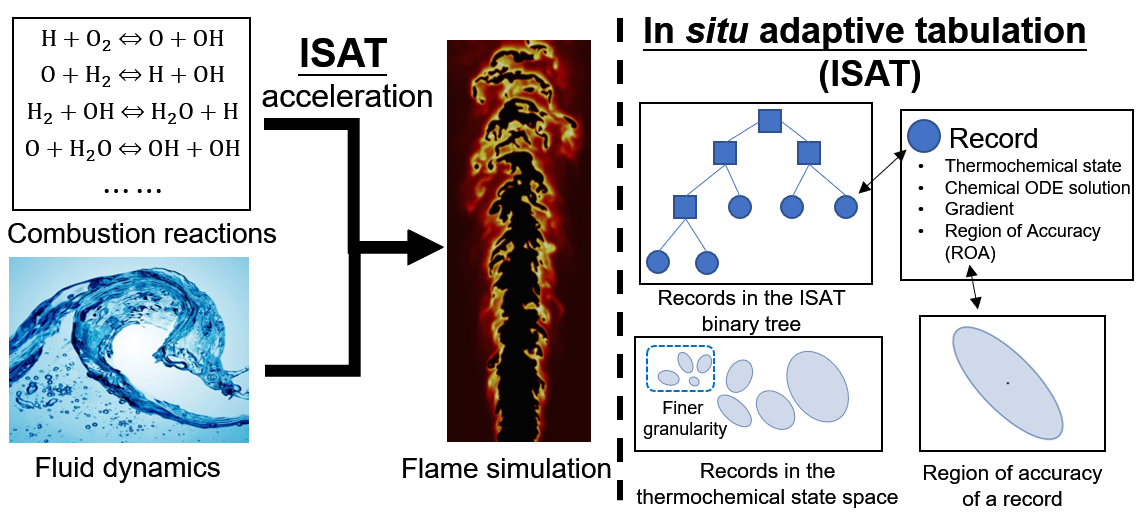
\includegraphics[width=0.80\linewidth]{ISAT schem.png} 
\caption{Schematic of turbulent flame simulation and ISAT.}
\label{ISAT_Schematic} 
\end{figure}


\section{Method}
\subsection{shared memory architecture}
In the proposed model, the primary objective is to optimize the utilization of compute nodes' resources effectively. To achieve this goal, I need a hybrid architecture that seamlessly integrates shared memory capabilities into the system's design. While there are various approaches to implementing shared memory functionality, one common choice is the hybrid MPI-OpenMP model, which leverages OpenMP for shared memory support and MPI for process-level parallelism across nodes. The hybrid MPI-OpenMP model has seen widespread use in parallel computing \cite{ouro2019scalability,he2020structured,zhong2020efficien}.

In the MPI-3 standard, the MPI Shared Memory (SHM) \cite{brinskiy2017introduction} is introduced for supporting shared memory address space among MPI processes on the same node. With the MPI SHM model, an innovative hybrid programming approach combining MPI and the MPI Shared Memory (SHM) model emerges (hybrid MPI-MPI)\cite{hoefler2013mpi+}. Both MPI-MPI and MPI-OpenMP models can use the shared memory to reduce communication time in one node. However, due to extra overheads from shared memory threading, hybrid MPI-OpenMP implementation may hardly outperform the pure MPI implementation \cite{rabenseifner2009hybrid}. Hence, many CFD solvers only use the pure MPI model rather than the MPI-OpenMP model. For codes lacking OpenMP support, adopting the MPI-OpenMP model necessitates a comprehensive overhaul of the entire parallel structure to accommodate OpenMP. The use of the MPI-OpenMP model only requires incrementally adding OpenMP directives to the computationally intensive parts of the existing MPI code. However, given the complexity of modern large CFD code, such changes require a lot of careful debugging. In this regard, the hybrid MPI-MPI model proves more adaptable and portable.  It requires only minor adjustments to existing MPI code to introduce shared memory capabilities. Given this advantage, the MPI-MPI hybrid model will be used in this work. Since the model is relatively new, there are still insufficient tutorials. I hope that I can provide more experience in the use of this model to help future developers.

When using MPI model, we found the following three problems:
%The MPI SHM model is different from openMP in that MPI is inter-process communication. Each process has its own virtual memory space. This leads to three problems:



%1. 这使得同一个物理内存在不同进程下会出现不同的地址。这使得无法利用共享内存构建链表,树等复杂数据结构。
%2. 在MPI中,申请内存是一个collective call,申请共享内存需要所有核心一同完成,这使得在运行过程中动态分配内存会使性能退化到串行代码。
%3.而且由于同步的机制是为多线程设计的,这使得MPI共享内存的同步缺乏工具。
%我们提出了一个解决方案, 我们在一开始申请一整块内存,对于整块内存来说虽然在不同进程中地址不同,但是整块地址上的偏移量是相同的,我们使用相对于首地址的偏移量来代替地址。我们自己实现了slab allocator,来自己管理内存,共享内存只在代码开始运行时进行一大块内存。之后不在申请共享内存。

\begin{description}
\item [1. Dynamic shared memory allocation] Dynamic shared memory allocation in MPI standard is a collective call executed by all processes, which means that a single process cannot allocate shared memory. However, when using the ISAT method, every processor should be able to update the table independently. If every update requires all the processes to allocate memory together, the efficiency of the whole system will be severely slowed down.
  \item [2. Memory address inconsistency] In modern operating systems, each process has its own virtual address space, which causes that for one block of physical memory, it can have different addresses in two processes. MPI SHM model is process-based rather than thread-based (in contrast, OpenMP is thread-based). Hence, the addresses of shared memory cannot be passed across processes, which makes the pointer cannot be used. ISAT is built based on a binary tree, which depends on the indexing method of the pointer. 
  \item [3. Synchronization] Using shared memory, synchronization is important. If shared data are not protected properly, unexpected errors could happen, but most existing methods are designed for thread-based model. 
  %MPI standard does not provide flexible and efficient methods to protect shared memory.
\end{description}


When shared memory is employed solely for the purpose of optimizing data communication time, the problems mentioned above do not come into play. However, when the objective extends to sharing intricate data structures and executing highly concurrent queries, it becomes imperative to address these shared memory-related issues. In response to these problems, we introduce a comprehensive set of memory management techniques:


\begin{description}
      \item [1.] Instead of allocating dynamic shared memory when needed, we allocate a big chunk of shared memory at the beginning, and we implemented a custom memory allocator (slab allocator \cite{bonwick1994slab}) to manage the shared memory. The slab allocator can provide efficient memory allocation for different sizes of objects and is now widely used by many Unix and Unix-like operating systems including FreeBSD and Linux. 
      \item [2.] Although a memory Byte in two processes may have distinct virtual addresses, the address offsets between memory Bytes from the same block remain consistent across processes. This consistency enables us to employ the offset relative to the initial address of the entire memory block as new addresses that can be used by shared memory
      \item [3.] C++ provides build-in atomic variables. The synchronization for atomic variables is done at the instruction level. As a result, Atomic variables are safe in a multi-threading environment as well as a multi-process environment.
Based on the atomic variable, mutual exclusion locks (mutex) are easy to implement. A mutex is a synchronization primitive: a mechanism that enforces limits on access to a resource when there are many threads/processes of execution. With mutexes, shared data can be protected from being simultaneously accessed by multiple threads/processes.
      
     % which is free from data races; that is, if one thread writes to an atomic object while another thread reads from it, the behavior is well-defined. Although this technique is used on multi-thread rather than multi-process code, we tested and found atomic variables also work in MPI. Based on the atomic variable, mutual exclusion locks (mutex) are easy to implement. A mutex is a synchronization primitive: a mechanism that enforces limits on access to a resource when there are many threads of execution. With mutexes, shared data can be protected from being simultaneously accessed by multiple threads.
    \end{description}

%



\subsection{Concurrent binary tree}
A challenge of developing the proposed shared-memory parallel ISAT is to ensure high efficiency and thread safety when manipulating the records in the table. A concurrent binary tree is implemented to ensure high performance. In simulations, most of the query can be directly retrieved from the table, which is a read operation.
Write operations (growth and addition) are performed when the existing data is insufficient. %Since there are far fewer read operations than writes operations, the concurrent binary tree, needs to be optimized for high-concurrency and high-performance reads, and low-concurrency writes.

Multiple reading operations can be performed simultaneously without causing corruption, but making writing operations paralleled are much more difficult. Improper ways can lead to unexpected errors. To ensure high efficiency and thread safety, the concurrent binary tree is designed to have the features below.

\begin{itemize}
    \item Reads are lock-free (reading processes never block, even while writes are ongoing)
    %\item Reading processes always see a consistent version of the tree
    \item Reading processes do not block writing processes
    \item Processes trying to write the same tree leaf block each other but never block reading threads
\end{itemize}


A mutex is used to block the node when a writing operation is executing. Hence, mutliple writing operation can be conducted at different tree nodes. As shown in the features, for better performance, the ISAT allows reads and writes to happen simultaneously. To achieve this, three techniques are used for this purpose: 1. During writing, the structure of the binary tree needs to be accessible. Specifically, addition and growth operations are shown in Fig.\ref{MPI_op}. When updating the tree structure, edges that do not affect the search are updated first (Fig.\ref{MPI_op}-2). After the other updates are completed, the last remaining parts are updated with an atomic operation (Fig.\ref{MPI_op}-3). This way, the tree structure is always complete for read operations.
2. Rather than update the data in place, all changes need to be first written to a new tree node or tree leaf, then linked to the tree. Specifically, the growth operation of ISAT can be completed by directly modifying the record, in order to protect the integrity of the data, we will first save the updated result on a new leaf, and then replace the original leaf (Fig.\ref{MPI_op}-1 Growth).
3. After tree nodes and tree leaves are removed, they still could be read by some processes. Thus, removed data need to be kept unchanged until these reads are finished. Specifically, the deteted red record in Fig.\ref{MPI_op}-3 Growth operation are kept. In this work, all removed memory is kept unchanged until the calculation of the current time step is finished.

\begin{figure}[htbp]
    \centering
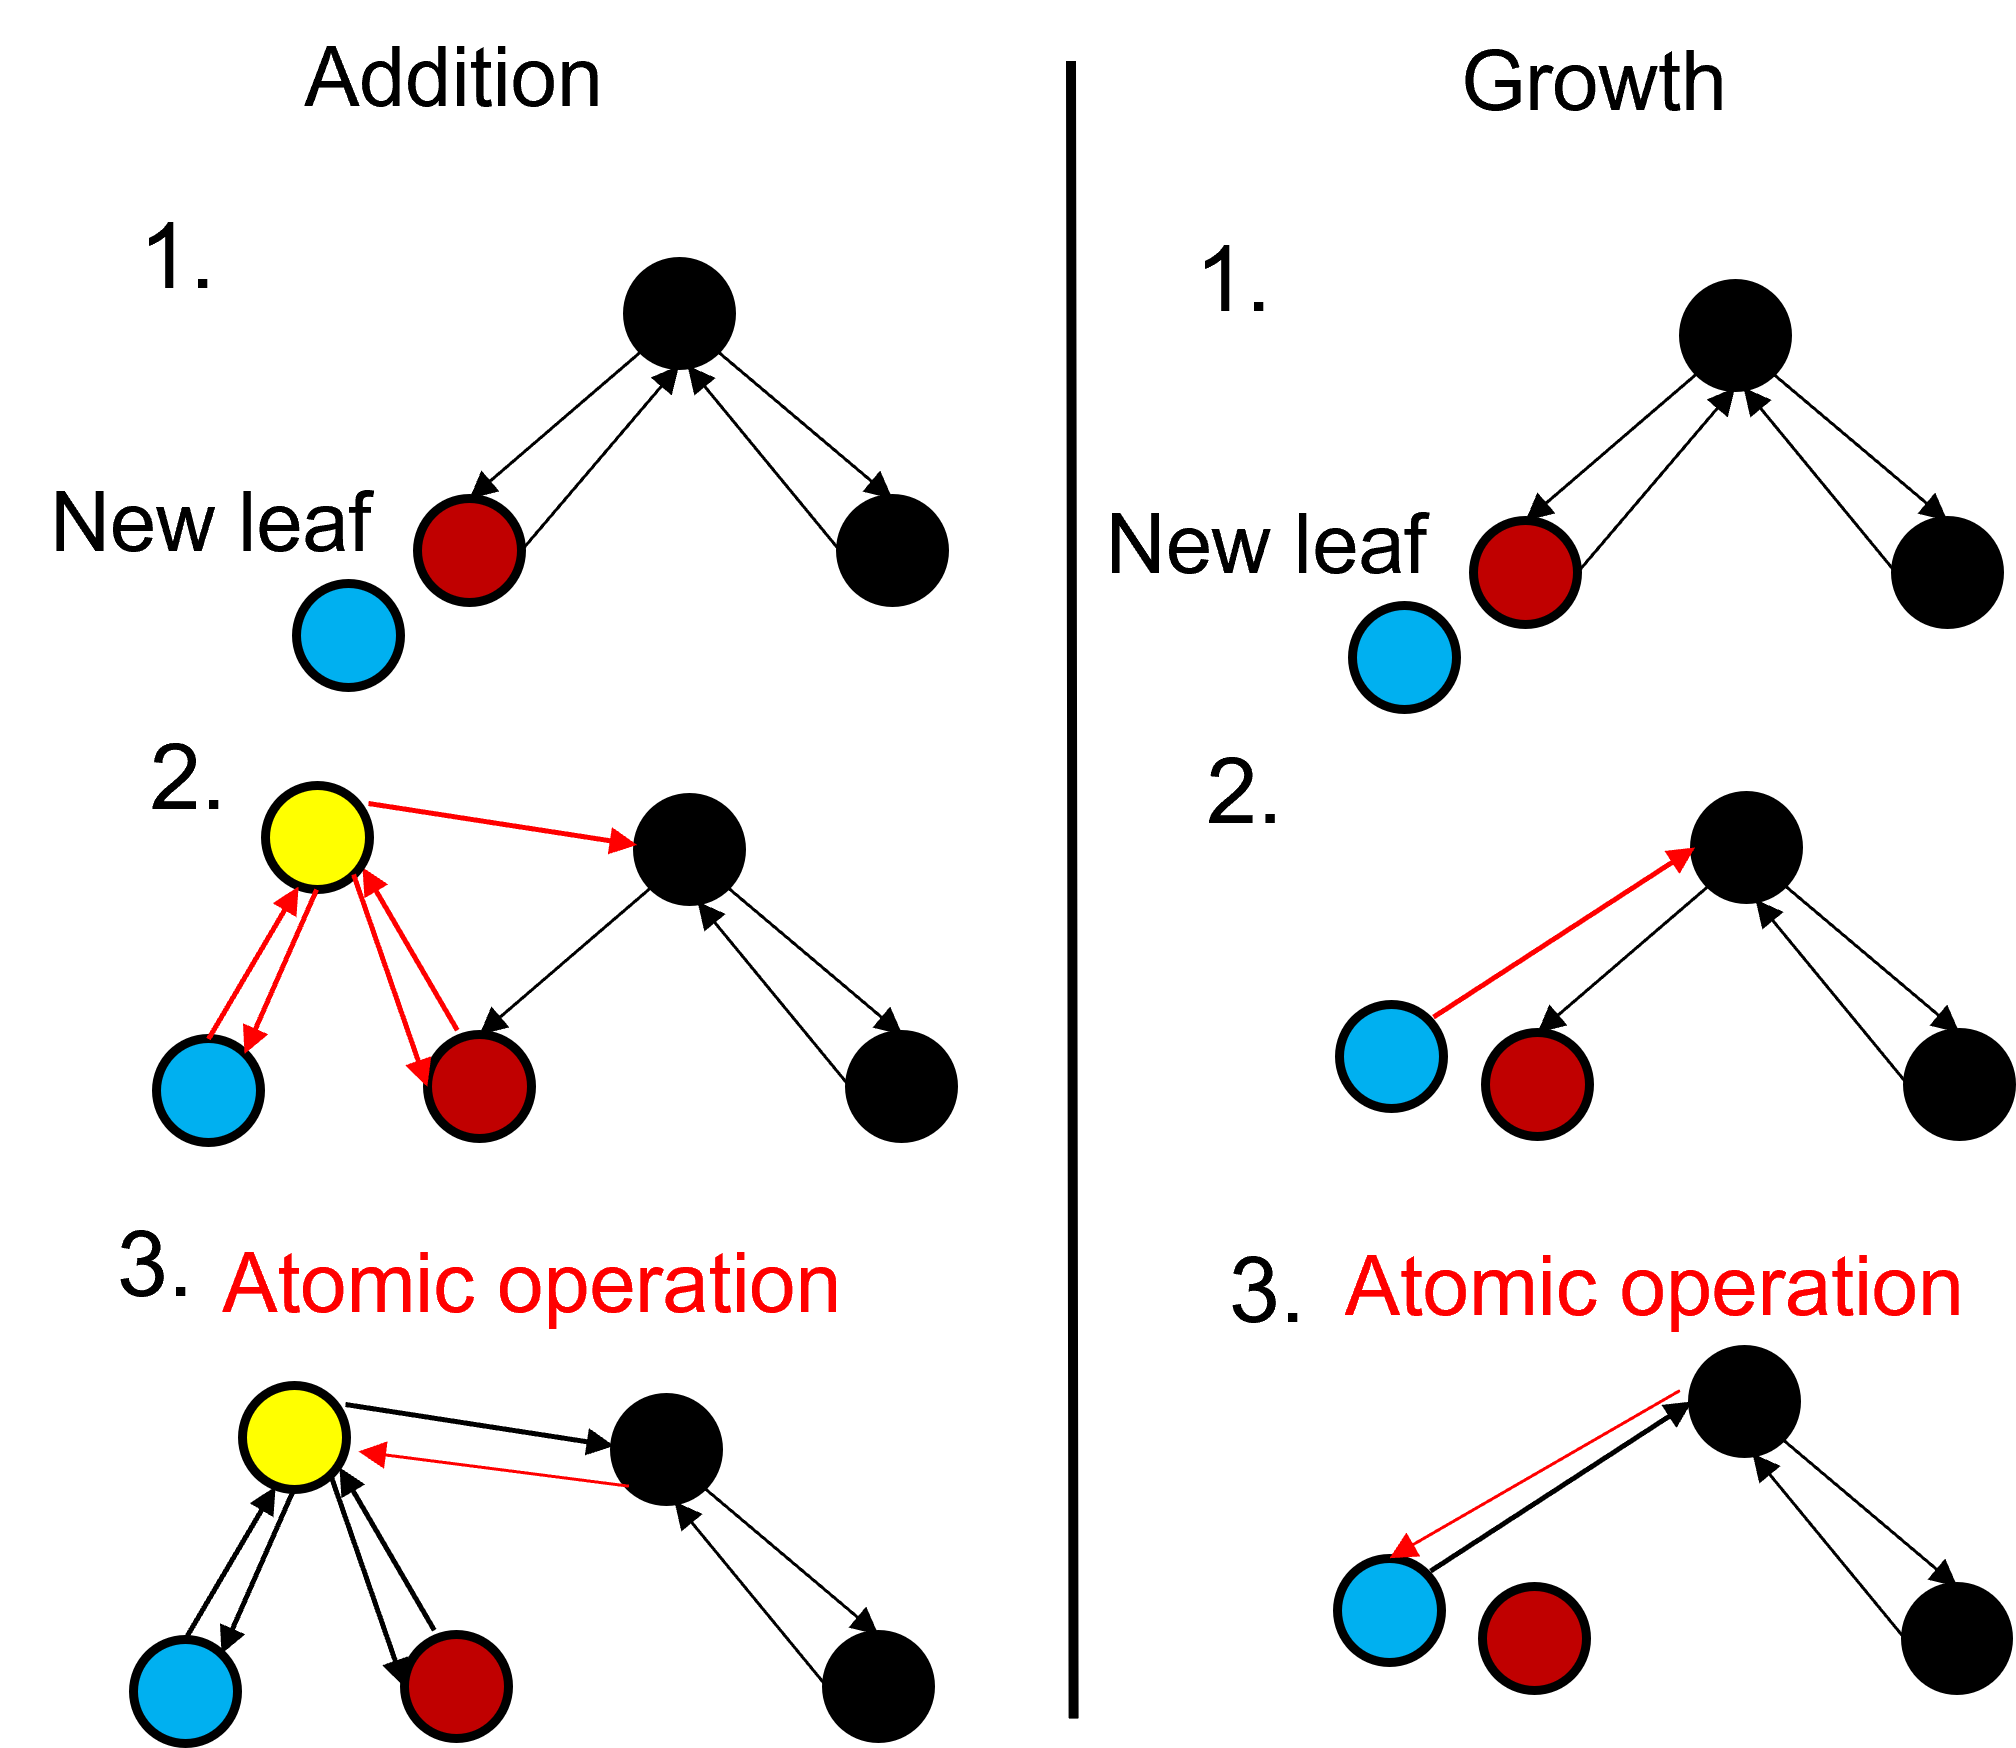
\includegraphics[width=0.9\linewidth]{tree_update.png} 
\caption{Schematic of concurrent binary tree opration. }
\label{MPI_op} 
\end{figure}


Although the tree structure supports multiple writes and reads at the same time, memory allocator is still a bottleneck. To handle this before each timestep, the allocator allocates a certain number of tree leaves and tree nodes for each process. In every timestep, we prioritize the utilization of pre-allocated memory, resorting to memory allocation through the allocator only when the pre-allocated memory is exhausted. This one-time allocation of a large memory block is exceptionally fast. By configuring an appropriate size for the pre-allocated memory, it becomes possible to eliminate the need for direct allocator usage in the majority of operations, without incurring excessive memory waste. This approach helps maintain a high level of parallelism throughout the entire algorithm.

Using the above method, we create a concurrent binary tree to store the ISAT table in each compute node. In this way, the data within a node can be centrally stored. Space wastage in multiple ISAT tables is avoided and unnecessary double calculations are reduced.

By employing the aforementioned approach, we establish a concurrent binary tree structure to store the ISAT table within each compute node. Through this method, all records within a node can be stored centrally, effectively mitigating space wastage in oringal ISAT method in which every process has its own ISAT table, and this way also reduces redundant calculations.

%使用上述方法,我们在每个计算节点建立一个Concurrent binary tree,用以存储ISAT table. 这样一来,一个节点内的数据都可以集中化的存储。避免了在多个ISAT表时的空间浪费,减少了不必要的重复计算。 

Regarding the redundant record deletion techniques discussed in the preceding section, implementing a highly concurrent linked list can prove challenging. Therefore, we opt for a simplified solution where we log the call timestamp after each record usage. Since identical timestamps are used for calls occurring within the same timestep, this approach effectively eliminates data race concerns without compromising performance. Periodically, at specified intervals of timesteps, we proceed to sort all records based on the timestamp and subsequently apply deletion criteria as previously defined.

In comparison to the original method, this approach has its drawbacks, particularly in terms of not being able to strictly guarantee conditions in every timestep. Additionally, the sorting operation encompasses all data, whereas the original method only affects incremental data. Consequently, this approach exhibits limitations when dealing with extensive data volumes. Nevertheless, given the well-controlled table size within this application, it does not impose a significant performance penalty.

%对于上一节提到的redundant record deletion methods,那个数据结构难以实现高并发的版本,因此我们使用了一个简化的版本,我们在每次使用一个记录后记录调用的时间,由于这种读写在同一个时间不长内被写入的值都是一样的,不存在数据竞争的问题,此过程不会降低速度。我们在每一定的时间步长后,根据最近调用的时间将所有的记录排序,然后使用之前相同的条件做删除。此方法相比于动态方法的缺点是,无法严格保证条件的满足,而且排序是针对所有数据的,动态方法是只对增量数据有改动。当数据量很大的时候这一方法会展现缺点,但是因为表格大小在此应用中控制的较好,不会带来明显的性能损失。

\begin{figure}[htbp]
    \centering

\includegraphics[width=0.9\linewidth]{MPI arch.png} 
\caption{Schematic of the proposed parallel ISAT method.}
\label{MPI_arch2} 
\end{figure}

\subsection{Load balancing}

In simulations, substantial fluctuations in physical properties typically manifest in localized regions, such as shock waves and contact discontinuities. Compared to other regions, the computation in these regions tends to add more records in the ISAT table, often leading to pronounced imbalances when directly employing ISAT in parallel simulations. Researchers tried to address ISAT parallelization challenges in previous works\cite{lu2009computationally,wu2018parallel}, primarily by attempting to partition the computational workload within the computing domain into discrete chunks. They utilize the MPI communication mechanism to allocate these task chunks to individual MPI processes, ultimately achieving a more equitable distribution of computational load. However, the effectiveness of this approach hinges heavily on the spatial characteristics of the flow and the specific domain decomposition. Furthermore, the substantial volume of MPI communication involved can adversely impact ISAT performance.

In contrast, our approach in this study involves sharing ISAT tables in memory, obviating the need to account for flow spatial characteristics and domain decomposition during task allocation. When distributing tasks, we bundle multiple tasks into batches (batch size is 100 in this work)and distribute them across the MPI processes to maximize the utilization of all available computing resources. The load-balancing algorithm employed is outlined as follows:

%在模拟中物理性质剧烈波动通常会集中在小区域内,比如激波,接触间断面,这些区域往往会为ISAT表中添加更多的记录。这使得在ISAT在并行时往往导致明显不平衡。ISAT的并行问题在一些工作里也被讨论过\cite{lu2009computationally,wu2018parallel},他们主要尝试将计算域内的计算量进行不同的划分,利用MPI通信机制重新分配给各个MPi进程,最终使得计算量更为均衡。这一方法的使用高度依赖计算流动空间分布上的特征,以及计算域的分解方法,并且大量的通信降低了ISAT的性能。由于在本工作中,我们将ISAT表在内存中共享,这使得在进行的分配任务时不需要考虑流动的空间特性。我们在分配任务时将多个任务打包,分发到不同的核心中,最大化的利用全部的计算资源。负载均衡算法如下:


We employ multiple linked lists using shared memory to efficiently handle load balancing. Specifically, we employ three key lists: List E, denoting "empty", serves as a repository for available empty nodes, while List T, denoting "task", is responsible for storing pending task inputs awaiting allocation. Additionally, each process maintains its own List F, signifying "finish," to store the output results.

Upon initialization, both List F and List T are left empty. List E is filled with nodes, with the number of nodes being three times the number of MPI processes. During this initialization phase, each process is marked as not idle.

%每个进程的计算域内的问题被分成一定大小的batch, 我们取batch size 为100, 
%在计算中需要使用多个共享内存存储的链表队列。empty队列用于存储空的节点,filled用于存储等待被分配计算的任务。每个进程有一个complete队列,用于存储计算完的结果。在初始化时,filled队列与complete队列被置为空。empty队列放置3倍的MPI进程数的node
%每个进程初始化为不空闲。

%\begin{description}
%%    \item [1.] Complete the calculation of the next batch
 %   \item [2.] Check whether the number of idle processes is greater than zero. If so, write the inputs of a certain number of batches of local tasks into List T. The number of batches is 2 times idle processes.
    %检查空闲进程数是否大于零。如果是,将接下来2倍空闲进程数个本地任务batch的输入写入共享内存,将其插入filled队列。
  %  \item [3.] Check whether list F for this process is empty. If the list is not empty, the task results are written to the corresponding computation domain, and the used node is inserted into list E.
    %检查本进程的complete队列是否为空。如果不为空,将完成了的job结果写入本计算域的对应位置,完成后将队列插入empty队列。
   % \item [4.] If all the batches have been computed or allocated, go to step 5, otherwise go back to step 1.
    %如果所有的sbatch都被计算或被分配出去了,进入第5步,否则回到步骤一
    %\item [5.] If this process is marked as idle and list T is not empty, fetched a batch from list T, finish the computing tasks, and place the result in the list F of the corresponding process.
     %如果本进程标记为空闲且filled队列不为空,取出一个batch,求解job,然后将结果放入对应进程的complete队列中。
    %\item [6.] Check whether list F for this process is empty. If the list is not empty, the task results are written to the corresponding computation domain, and the used node is inserted into list E.
    %检查本进程的complete队列是否为空。如果不为空,将完成了的job结果写入本计算域的对应位置,完成后将队列插入empty队列。
    %\item [7.] If the process is not idle, it is marked as idle, and the number of idle processes increases by one.
    %如果进程不空闲,将其标为空闲,空闲进程数增加一。
    %\item [8.] If the number of idle processes is equal to the total number of MPI processes, the results of all tasks of this process are written back and the list T is empty, the calculation ends. Otherwise, go back to step 5.
    %如果空闲进程数等于进程总数,本进程全部任务的结果写入存储位置,且filled队列为空,结束计算,否则回到第5步
%\end{description}

%\begin{algorithmic}
%Complete the calculation of the next batch
%Check whether the number of idle processes is greater than zero. If so, write the inputs of a certain number of batches of local tasks into List T. The number of batches is 2 times idle processes.
%\end{algorithmic}   


\RestyleAlgo{boxruled}
\LinesNumbered
\begin{algorithm}[H]
    \caption{Load balancing algorithm} \label{al:LB}
    List F and List T are left empty \;
    List E is filled with $N$ empty nodes, $N = 3 \times N_{process} $ \; 
    idle $\gets$ false\;
    $N_{idle} \gets 0$\;
    \While{number of allocated batches $<$ number of total batches}{
        Complete the calculation of the next batch\;
     \If{$N_{idle} > 0$}{
        write the inputs of $2\times N_{idle}$ batches of local tasks into List T\;
      }
      \If{list F of rank R is not empty}{
        the task results are written back to the corresponding computation domain\;
        the used node is inserted into list E\;
      }
    }
    \While{ idle = true \textbf{and} $N_{idle }=  N_{process}$ \textbf{and} list T is empty }
    {
        \If{idle = true \textbf{and} list T is not empty}{
        idle $\gets$ false\;
        $N_{idle} \gets  N_{idle} - 1$\;
    fetched a batch from list T\;
    finish the computing tasks\; 
    place the result in the list F of the sender's process\;
    }
    \If{list F of rank R is not empty}{
        the task results are written back to the corresponding computation domain\;
        the used node is inserted into list E\;
    }
    \If{idle = false}
    {
        idle $\gets $ true\;
        $N_{idle} \gets   N_{idle}$ + 1\;
    }
    }
\end{algorithm}



\begin{figure}[htbp]
    \centering
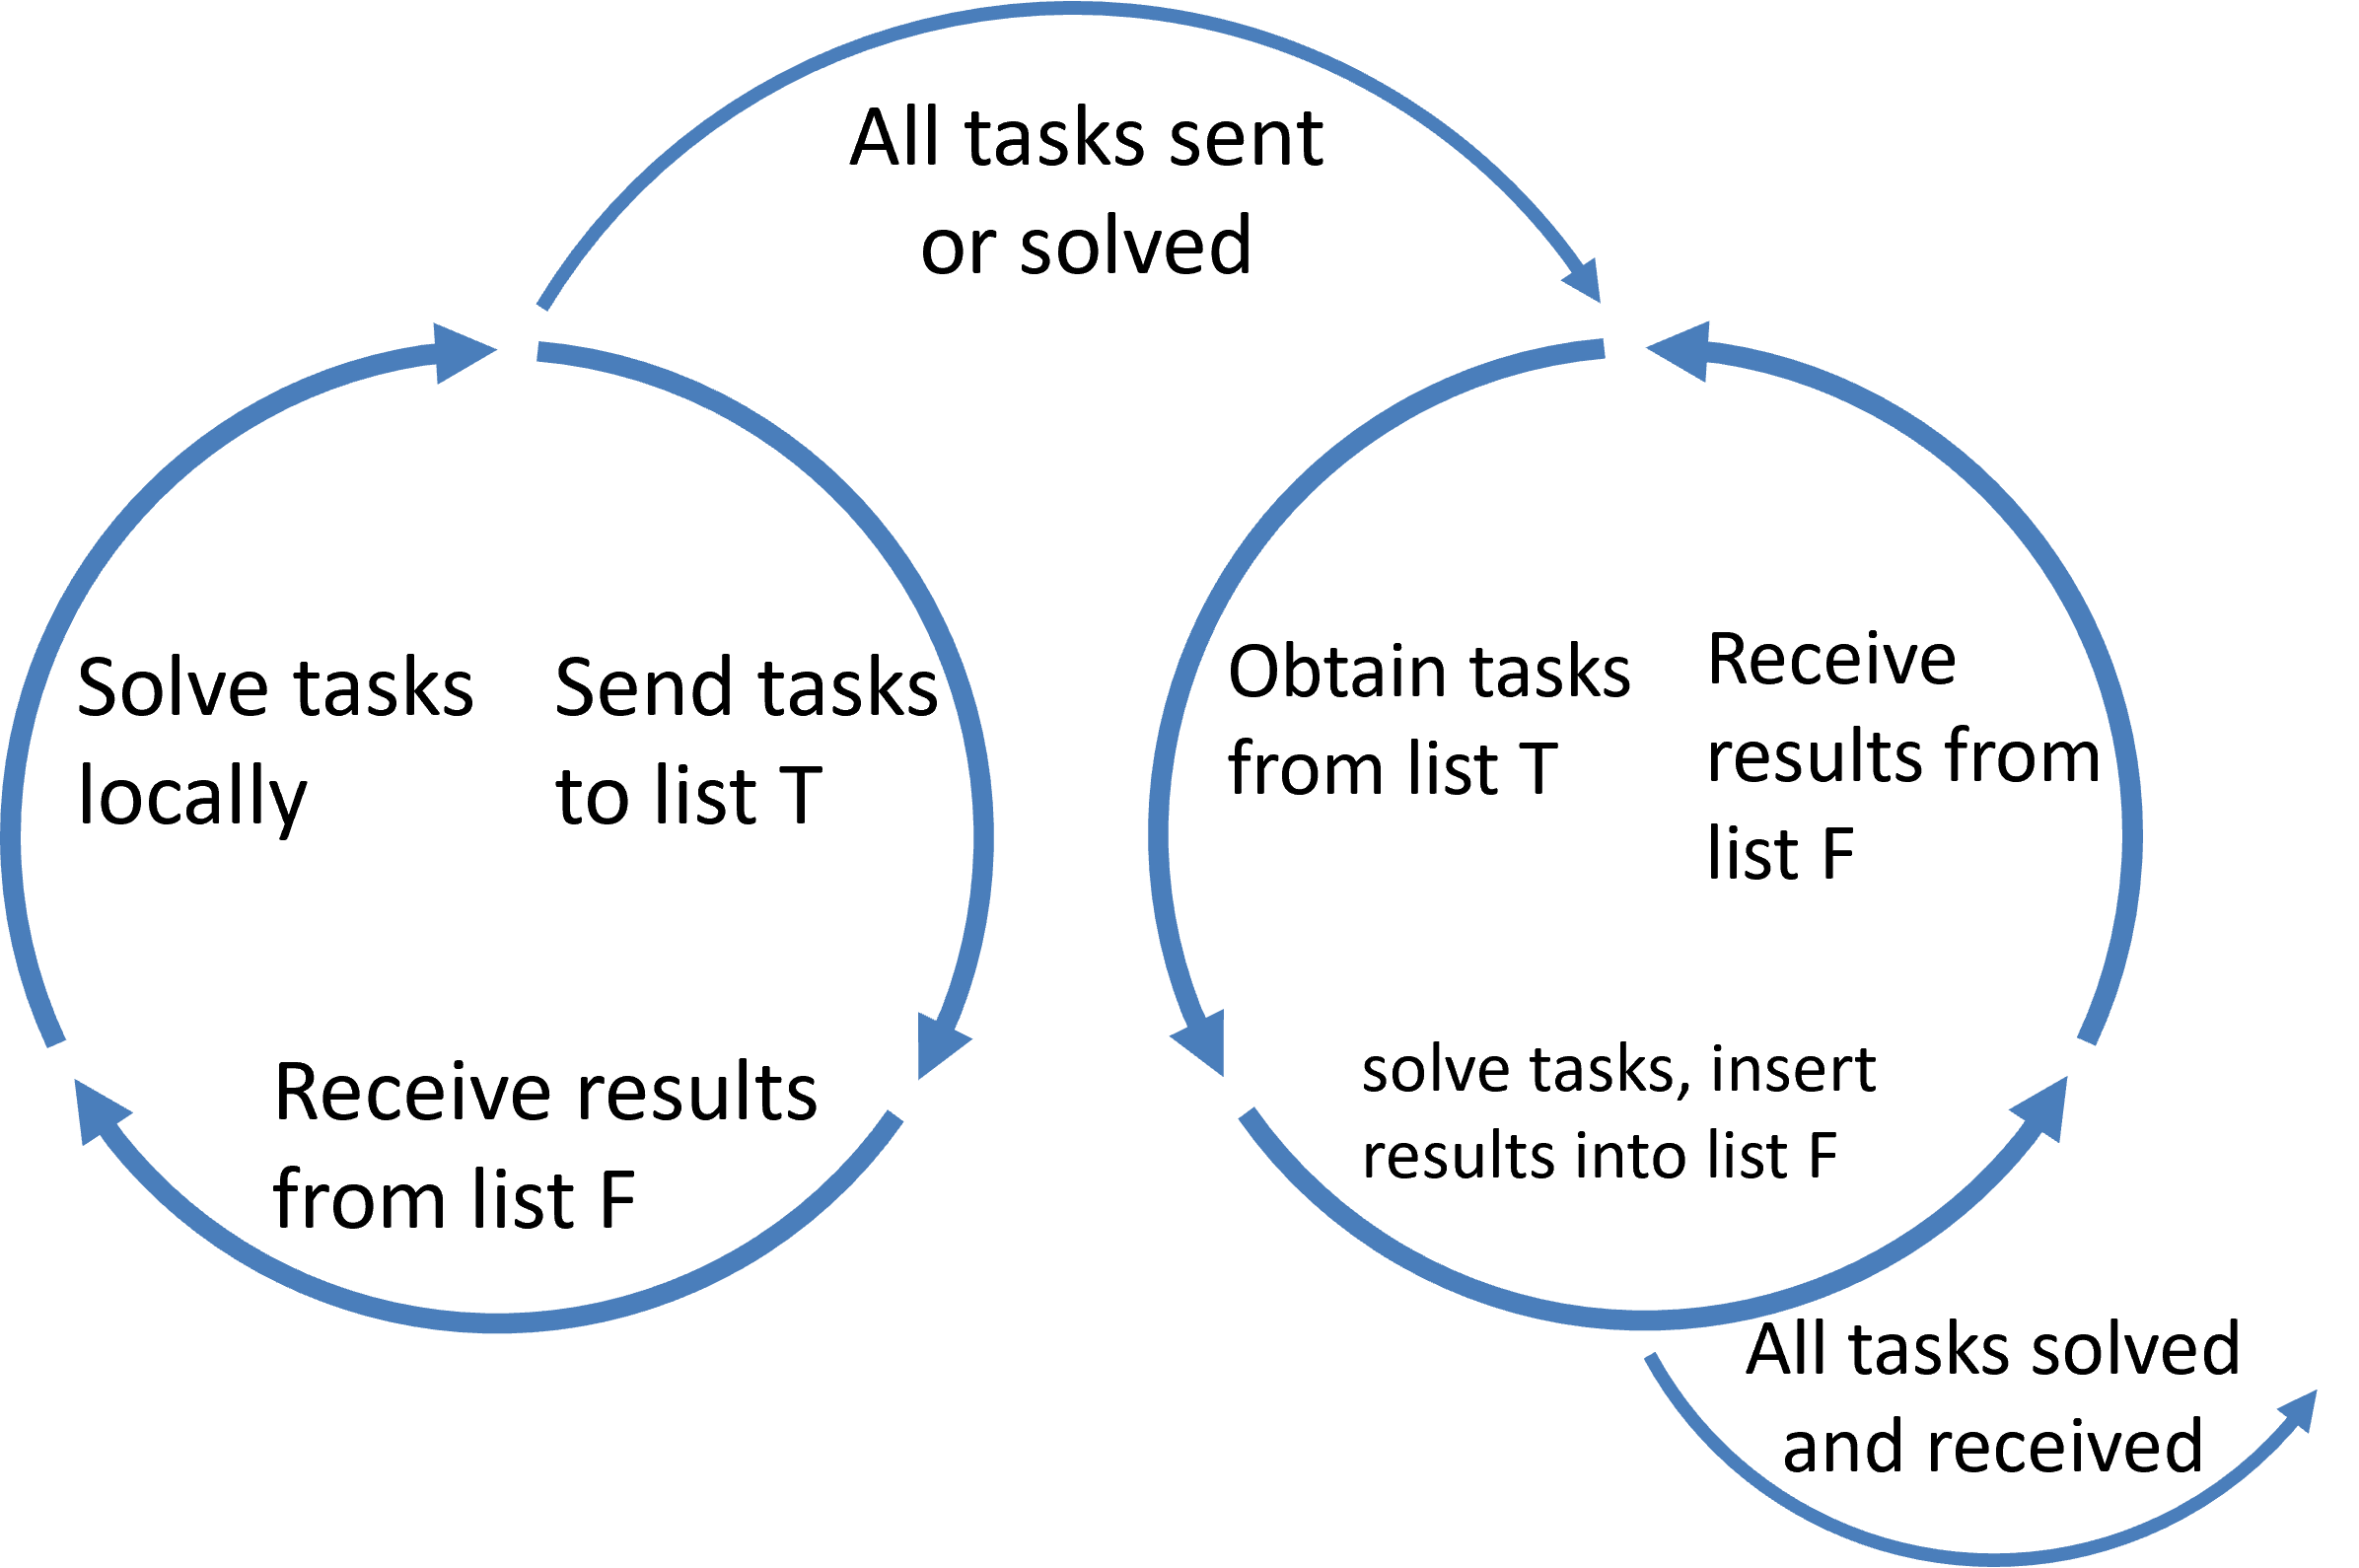
\includegraphics[width=0.9\linewidth]{LB_chart.png} 
\caption{Schematic of load balancing algorithm}
\label{MPI_LB} 
\end{figure}


In Algorithm \ref{al:LB}, Line 5 to 14 constitute a local computation and task allocation loop, while Line 15 to 31 encompass a loop for solving shared tasks and writing back the output. In simulation, the slow processes are mainly in the first loop, and the faster processes quickly complete their tasks and enter the second loop to share the computation tasks of the former, (see in Fig. \ref{MPI_LB}).  %Because the ISAT tables are shared among all processes, every process updates the same ISAT table, irrespective of the computational domain.
It's crucial to emphasize that linked list operations must address data race issues, necessitating the use of mutexes to guarantee the safety of each operation. Fortunately, these operations involve minimal computational overhead, resulting in negligible performance impact.
Through the method outlined above, all tasks can be equitably distributed across all processes, thereby maximizing the efficient utilization of computing resources.
%1-4是一个本地计算和任务transfer循环,5-8是求解被共享的任务,与将输出存储的循环。由于ISAT表是共享的,所以任何一个进程都能ISAT表都是相同的,不受计算域影响。需要强调的是队列操作需要处理数据竞争的问题,每次操作都需要用mutex保证操做的安全。这样的操作由于需要的计算量非常小,mutex的使用几乎不会产生对性能的影响。通过以上的方法所有任务可以被均匀的分配给所有的进程,最大化的利用计算资源。


\section{Results}

\subsection{2D shockdroplet simulations}

%我们使用了在之前章节使用的shock-droplet interation simulation,选取FC这一算力,对这一新模型的性能进行测试,首先我们测试了将计算域分为在x方向上分为两部分,两个MPI进程分别叫做P1,P2,
%We used the shock-droplet interaction simulation using the FC scheme in the previous chapter to test the performance of the new models. First, we used two processes to conduct the simulation. We decomposed the domain into two parts in the x direction. The two MPI processes are called P1 and P2, as shown in Fig.~\ref{MPI_P2}.

In the preceding chapter, we harnessed the power of the FC scheme to simulate the interaction between shockwaves and droplets. This simulation served as a crucial testbed for evaluating the performance of novel models. To carry out this investigation, we first conduct a simulation using two MPI processes. In the x-direction, we decomposed the domain into two distinct regions, aptly named P1 and P2, as illustrated in Fig.~\ref{MPI_P2}. We applied three ISAT methods for the simulation: the original ISAT approach (where each process generates its independent ISAT table), a shared ISAT approach, and a shared ISAT with Load Balancing (LB).
\begin{figure}[htbp]
    \centering
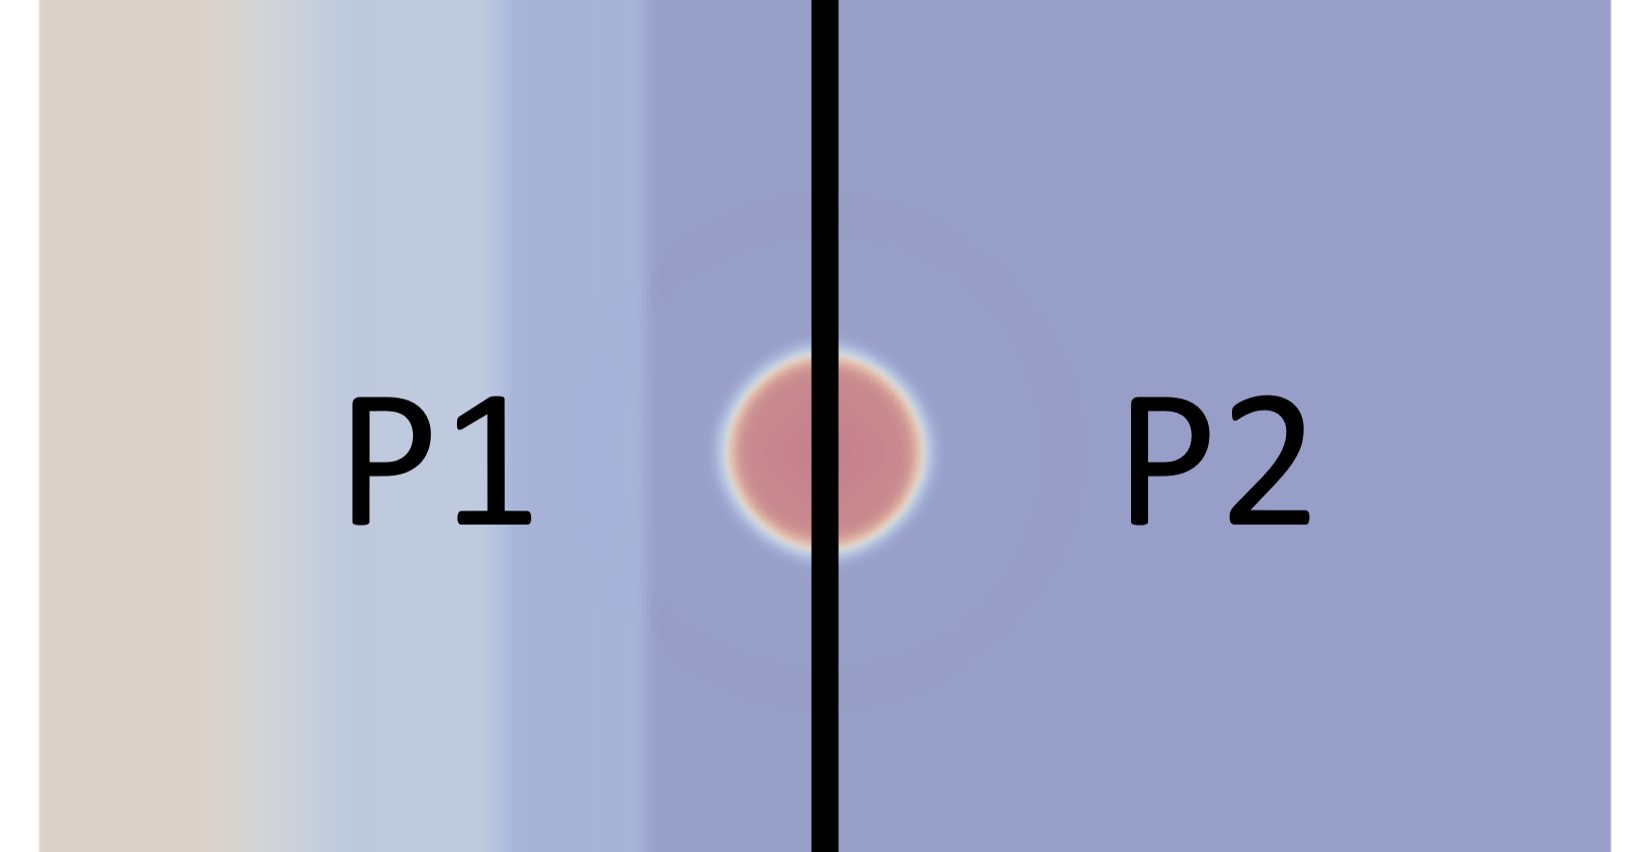
\includegraphics[width=0.\linewidth]{P2_2.png} 
\caption{Schematic of comuputation domain in  two-process simulation}
\label{MPI_P2} 
\end{figure}



In Fig.\ref{MPI_2core}, we present the CPU time and memory consumption (in terms of table size) used during the execution of these simulations utilizing the three ISAT methods. In Fig.\ref{MPI_2core}(a), load imbalance is evident for both the shared ISAT and the original ISAT. This disparity starts at the initial encounter of the shockwave with the droplet in P1, occurring at approximately t1 (around 0.5 $\mu s$). This event precipitates a surge in computational workload within P1. Meanwhile, P2 remains unaffected until approximately 0.7 $\mu s$ (as denoted by t2 in Fig.\ref{MPI_2core}(a)), at which point the shockwave enters P2's computational domain, leading to an increase in computational demand. At roughly 1.5 $\mu s$, the shockwave's impact on P1 diminishes, subsequently reducing CPU time. The shared ISAT approach with LB makes good use of computing resources, and both processes achieve precisely equal CPU times.

In order to compare parallel performance, we realize the slower process dictates the overall computational pace, necessitating that other processes wait until the slowest one completes its calculations. In each step, the slowest process determines the duration of computation. Comparing the three methods, we can see that the shared ISAT method shows better performance compared to the original ISAT. This improvement can be attributed to its ability to allow P1 and P2 to utilize each other's computation results, thereby mitigating redundancy. Moreover, the shared ISAT approach with LB further improves performance and minimizes load imbalance. Quantitatively, shared ISAT outperforms the original ISAT by 9.5\%, while shared ISAT with LB boasts a remarkable 34\% improvement in computational efficiency.


%我们使用三种方法分别进行模拟,分别是使用原先的ISAT(每个进程建立字节的ISAT表),共享的ISAT,共享的ISAT+ Load balancing (LB)。
%下图展示了我们使用三中方式进行模拟时,CPU time 与表格大小(内存消耗)。在a图上我们很清楚的看到,Shared ISAT 与 原先的ISAT有明显的不平衡。这一点也非常好理解,激波首先P1的区域内与液滴碰撞,导致计算量的增加,这是P2的计算域仍然是不受影响的,直到大约0.7mus时,激波进入P2的区域计算量开始增长。到大约1.5mus左右,P1内受激波的影响减少,CPU time 降低。可以看出shared ISAT比原先的ISAT性能有所提升,这是由于其共享特性P1,P2可以使用另一个进程的计算结果,减少了一些冗余计算。shared ISAT with LB 由于其算法特性导致两个进程的CPU时间完全一样。由于在并行中,较慢的进程是瓶颈,其他进程必须要等待直到最慢的进程完成。每个步长里最慢的进程是决定计算使用的时间。因此可以明显看到shared ISAT + LB 很明显的提高了计算速度。对于这个算例,shared总计算速度比ISAT快9.5\%,LB 比ISAT快34\%.
Fig.\ref{MPI_2core}(b) illustrates memory consumption through table size for three methods. In the original ISAT, we also provided separate table size data for process P1 and P2. Notably, the memory growth patterns for P1 and P2 align with CPU time growth. Around $1.5 \mu s$, P1's table size remains unchanged, which is because the redundant record deletion method works and limits the continued growth of table size.

The memory consumption of the two methods using the shared ISAT is similar. Throughout the entire computation process, the shared ISAT without LB consumes approximately 86\% of the memory space required by the original method, while with LB method, utilizes approximately 77\% of the original method's memory footprint.


%图b用table size展现了不同方法的内存消耗,在原先的ISAT中我们还额外画出了P1,P2两个线程分别的table size。P1,和P2的内存增长的区间很好地对应了CPUtime增长的部分。P1在1.5mus左右,table size 没有变化,这是因为redundant record deletion methods起作用了,限制了table size的继续增长。两个共享ISAT的方法的内存消耗比较接近。在整个计算中share方法与LB方法分别使用了原方法86\%,77\%的内存空间。

%下一部分,我们将算例分为四个进程,进一步观察分割方式对性能的影响

\begin{figure}[htbp]
    \centering
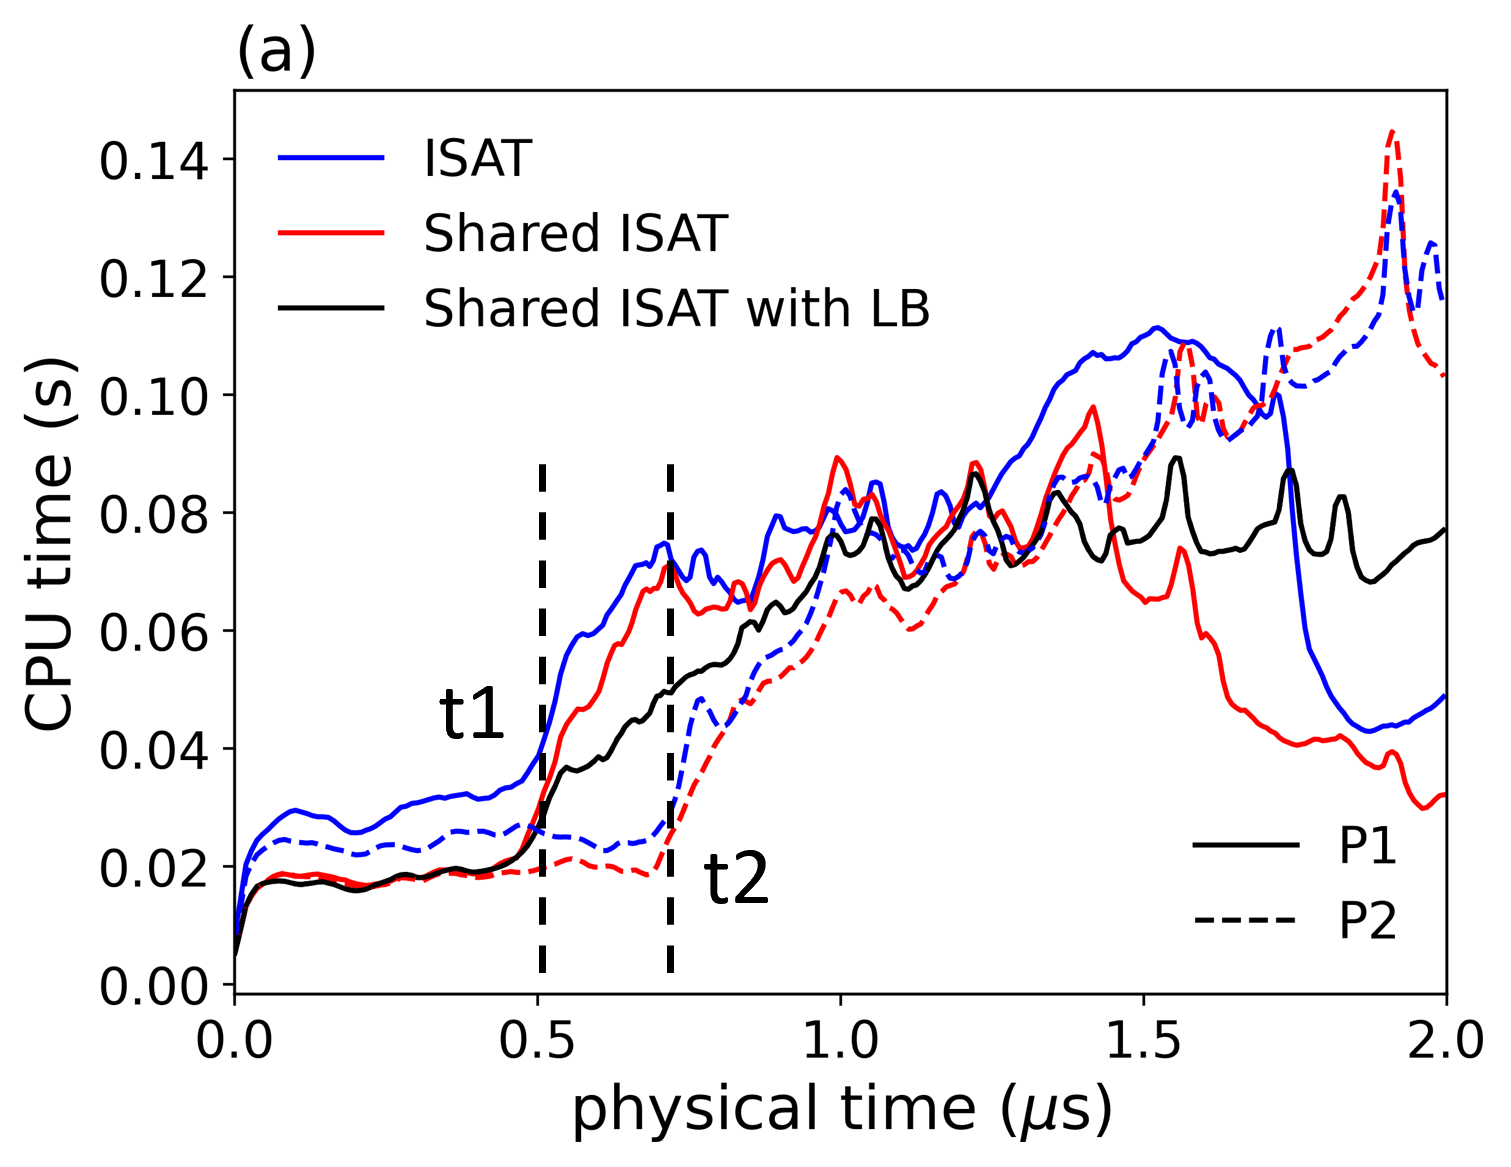
\includegraphics[width=0.45\linewidth]{2core_time_2.png} 
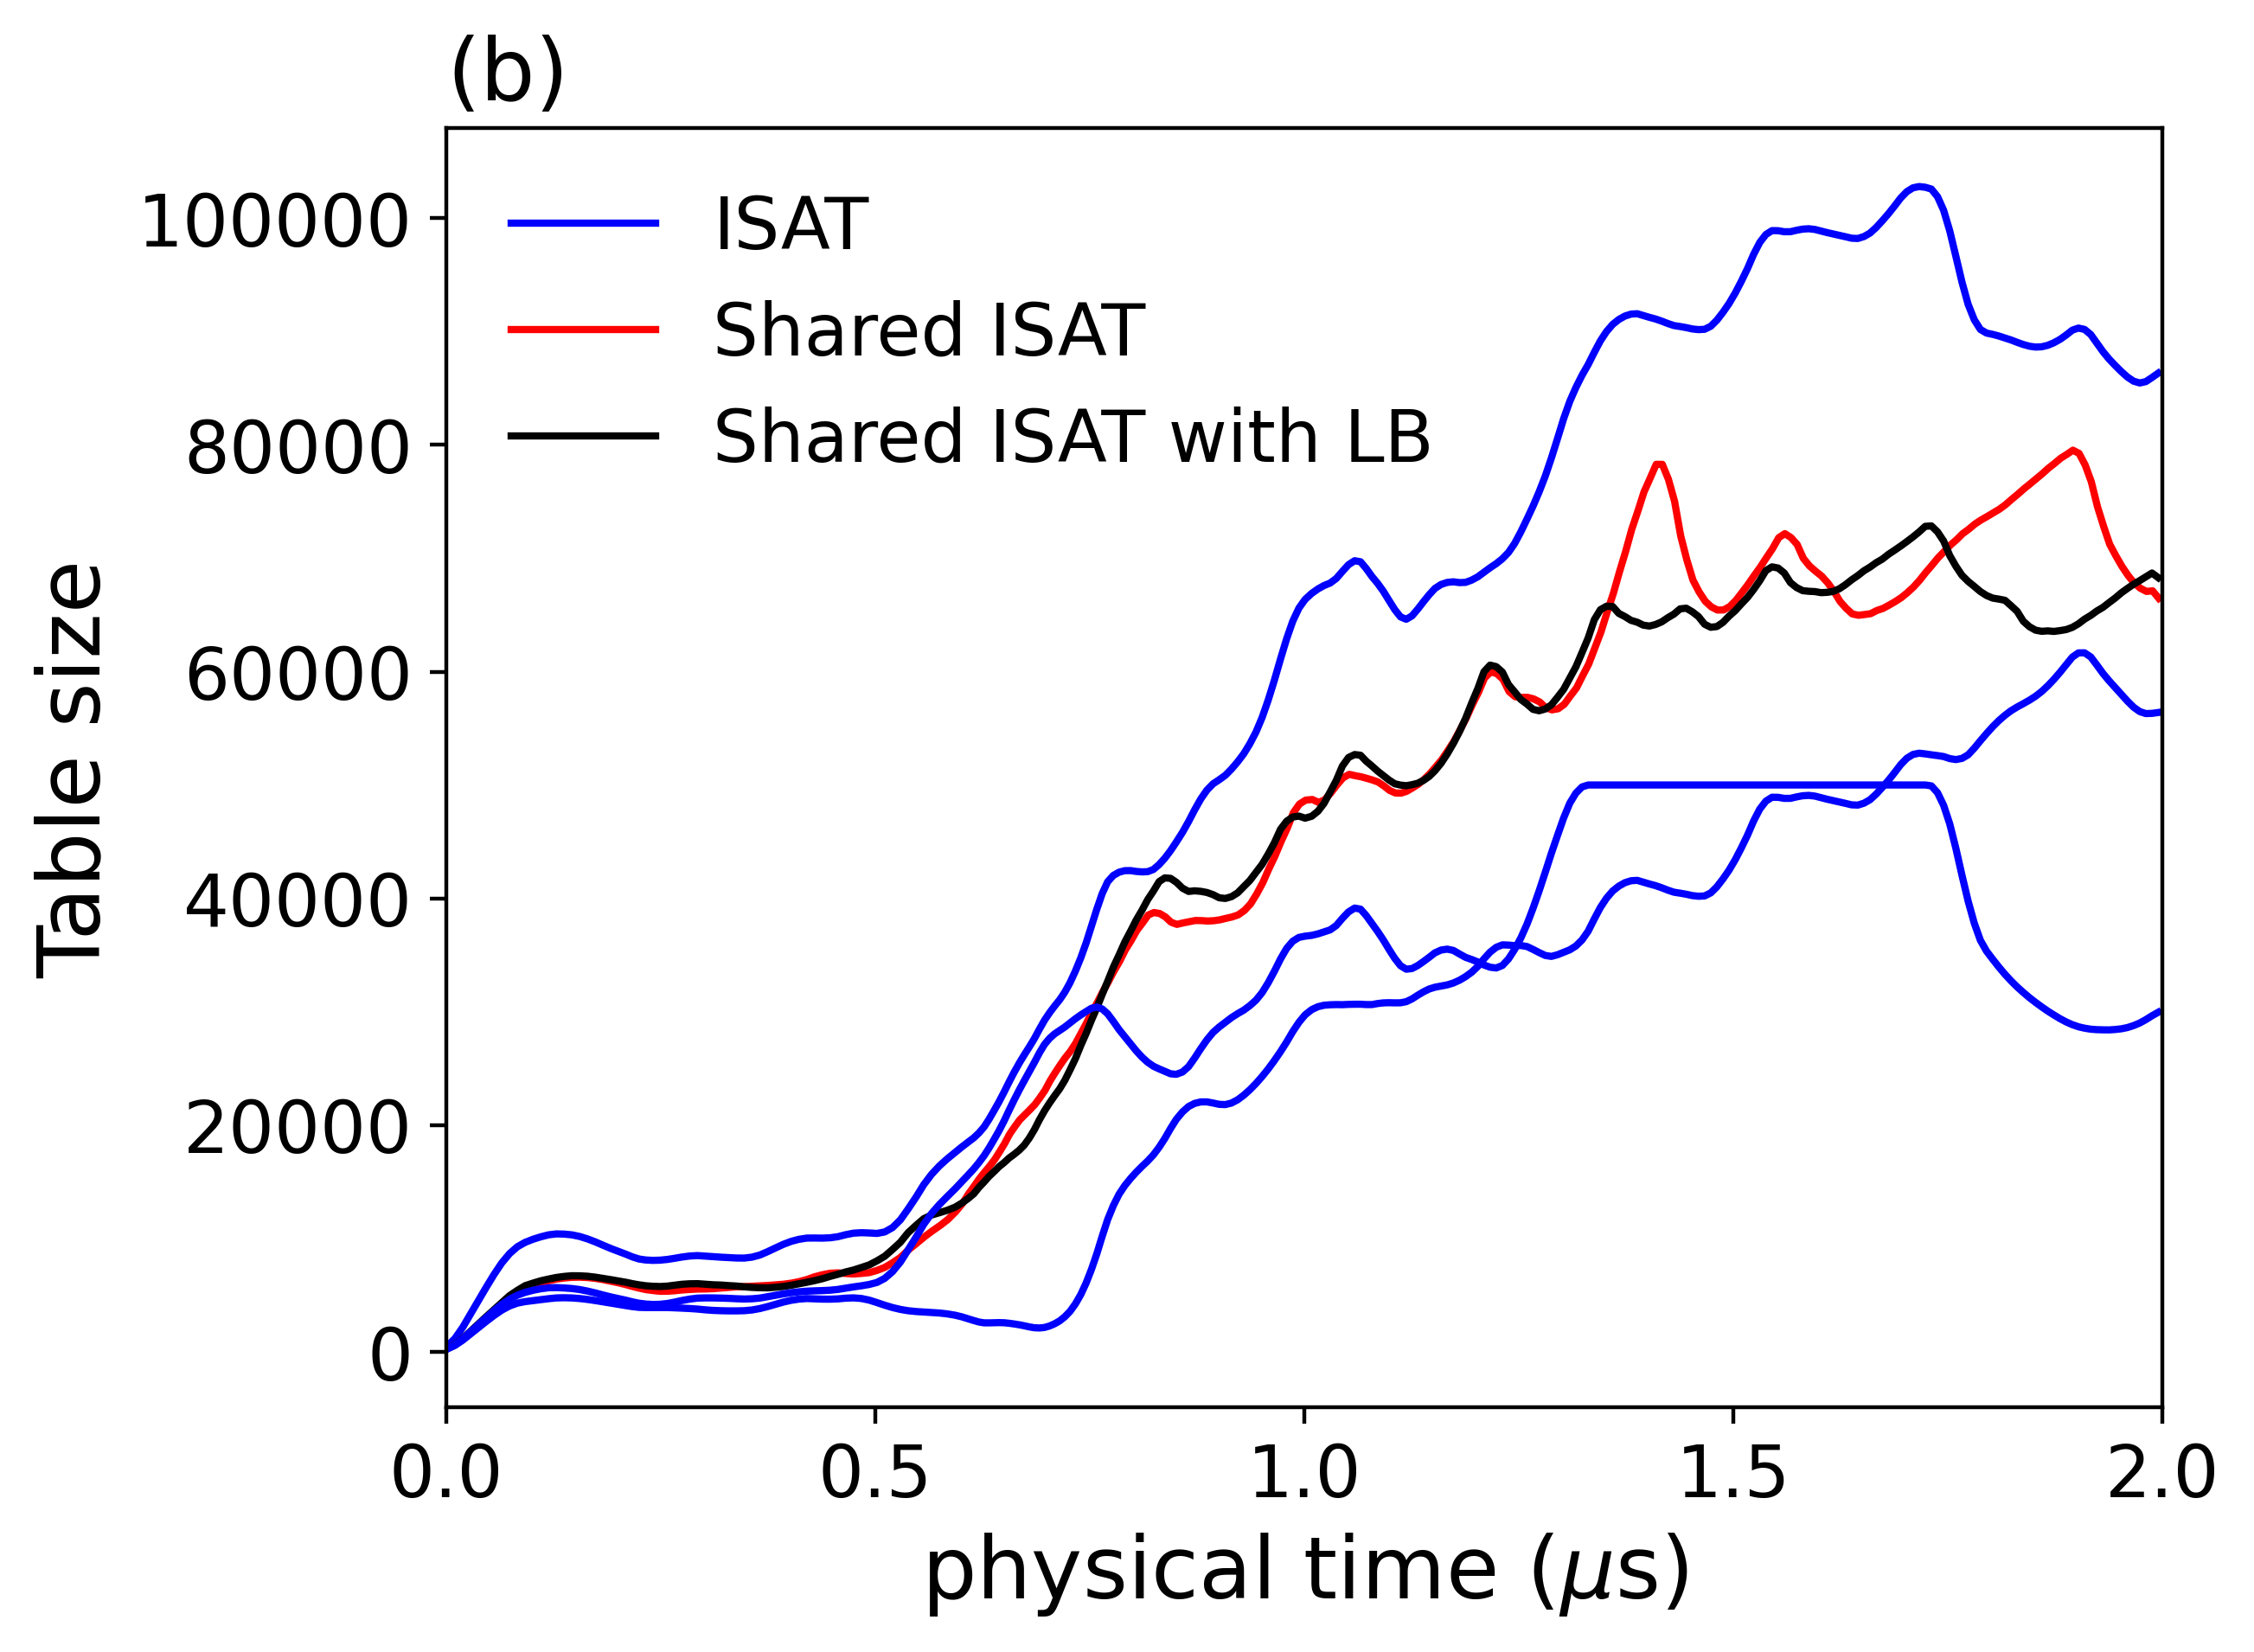
\includegraphics[width=0.45\linewidth]{mem_2core.png} 
\caption{(a) The performance of different ISAT methods, in terms of the CPU time spent in every time step. (b) Memory usage of different ISAT methods, in terms of table size at every time step.}\label{MPI_2core} 
\end{figure}

In the next part, we use four processes to further observe the effect of domain decomposition on performance.

%用4个MPI线程时,有三种常用的分解方式, 4x1 (在x方向分成4份,y方向分成一份,下同),2x2,1x4。 我们使用之前使用的三种IAST方法计算分别采用3种domain decomposition的方法模拟,得到9个结果。由于在之前的分析我们看到oringal ISAT和shared ISAT的不同进程在模拟中的CPU time趋势接近,我们在下图只展示oringal ISAT的结果。可以看到在4-1下,有两个进程几乎完全空闲,这是位于左右两侧的计算域,其中不含有液滴,于是内部的热力学状态十分简单,能够快速的查表计算。中间两个进程的情形比较接近之前两个进程的情形。在2-2下,这种情形相当于把上一节讨论两个进程的每个进程在在y方向均分,由于算例上下对称,这y方向分割,负载很均衡。在1-4下,最接近上下两侧的计算域完全不包含液滴,tabulation效率很高,只在reflection wave 进入其计算域时计算量提高。这三种方式里2-2的分割负载最为均匀。在shared ISAT with LB 中,三种分割方式对性能的影响明显较小。由于LB算法是有一定的开销的,2-2 这种更为均衡的分割方式性能更好一点。

When employing four MPI processes, there are three common strategies for decomposition: $4\times1$ (dividing the domain into four sections along the x-axis and one along the y-axis, the same applies below), $2\times2$, and $1\times4$. We conducted simulations utilizing all combinations of three ISAT methods and three decomposition techniques, resulting in a total of nine outcomes. Given that our previous analysis showed similar CPU time trends between the original ISAT and shared ISAT during simulation, we present only the results for the original ISAT in Fig.~\ref{MPI_4core}.

Observations reveal that when using a $4\times1$ decomposition, two processes remain largely inactive, positioned on the left and right sides (along x direction) of the computational domain. These regions don't contain liquid droplets and thus exhibit a straightforward thermodynamic state conducive to efficient tabulation. The results of the middle two processes closely resemble those of previous simulations (see Fig.~\ref{MPI_2core}(a)). In the case of $2\times2$ decomposition, this situation is very similar to the result of two processes. Because the computation domain of each process contains droplets, the computational load remains highly balanced.

In the $1\times4$ decomposition, the processes of the upper and lower domains contain no droplets. Consequently, tabulation efficiency is notably high. Additional computation is only required when the reflection wave enters their computational domain. Among the three decomposition methods, $2\times2$ achieves the most equitable load distribution. When employing shared ISAT with LB, the three decomposition methods exert less influence on performance. Given that the LB algorithm incurs a certain level of overhead, the more balanced $2\times2$ decomposition method delivers better performance.

\begin{figure}[htbp]
    \centering
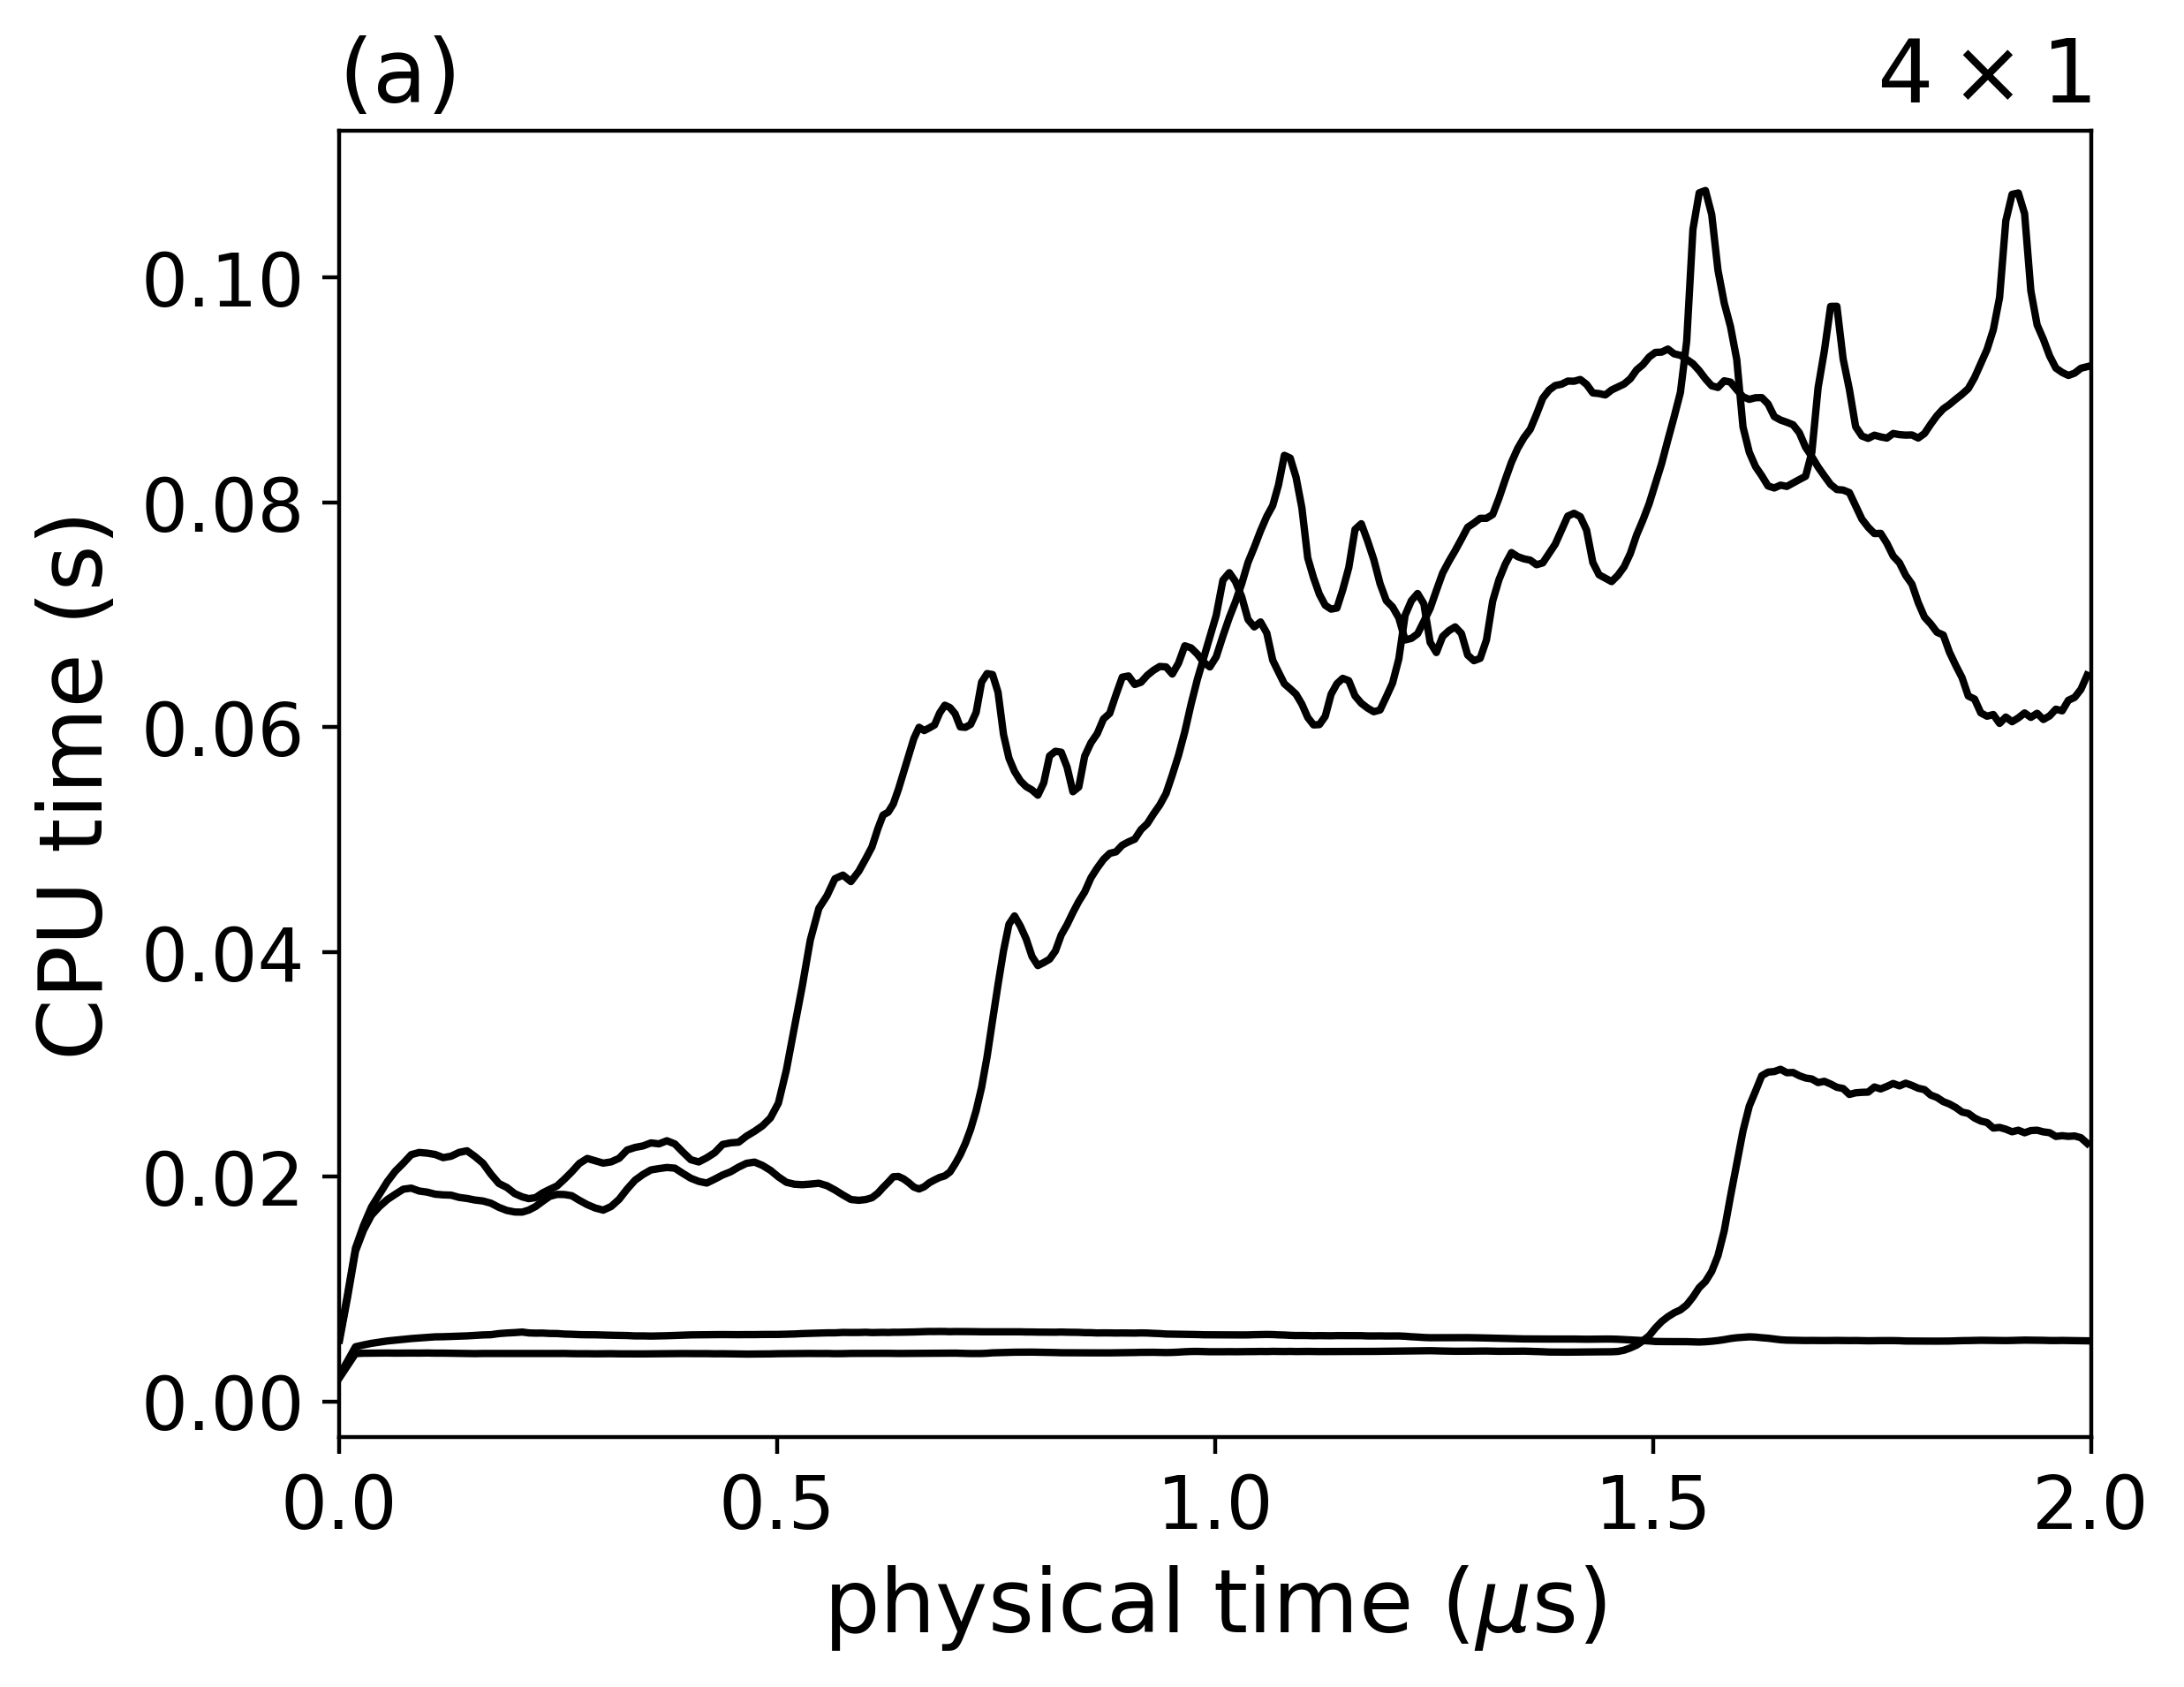
\includegraphics[width=0.45\linewidth]{time_4core_4-1.png} 
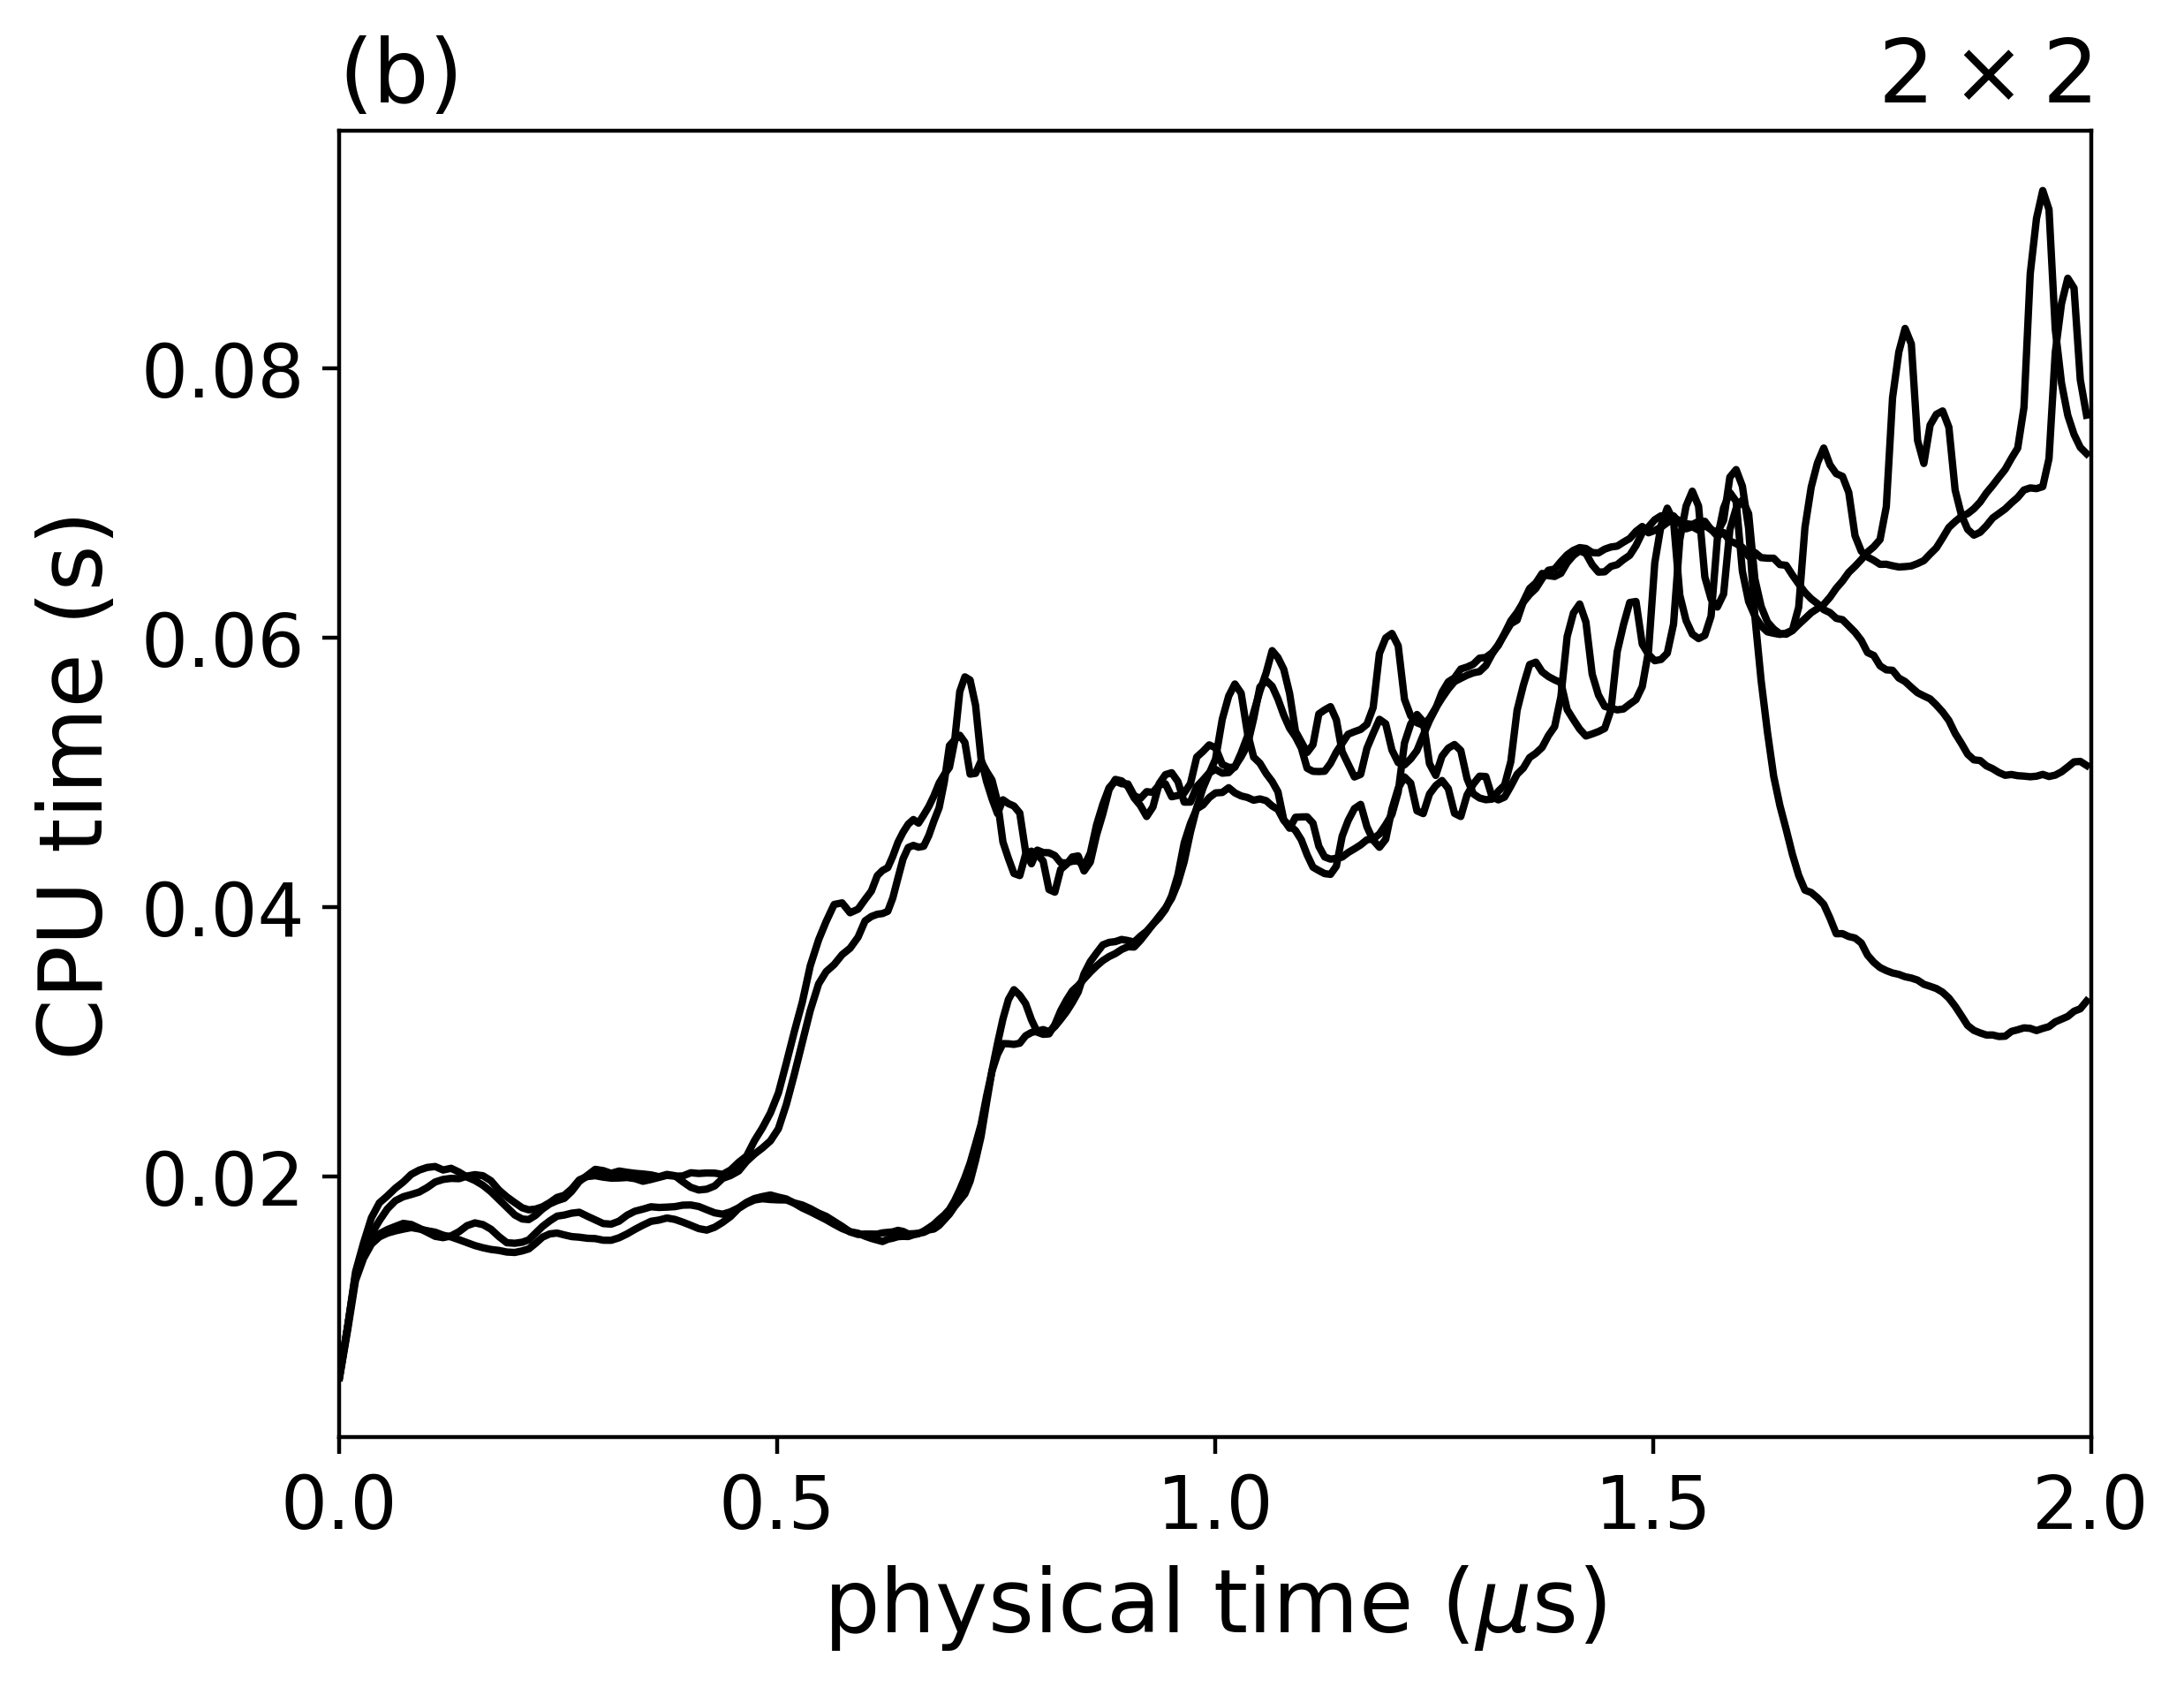
\includegraphics[width=0.45\linewidth]{time_4core_2-2.png} 

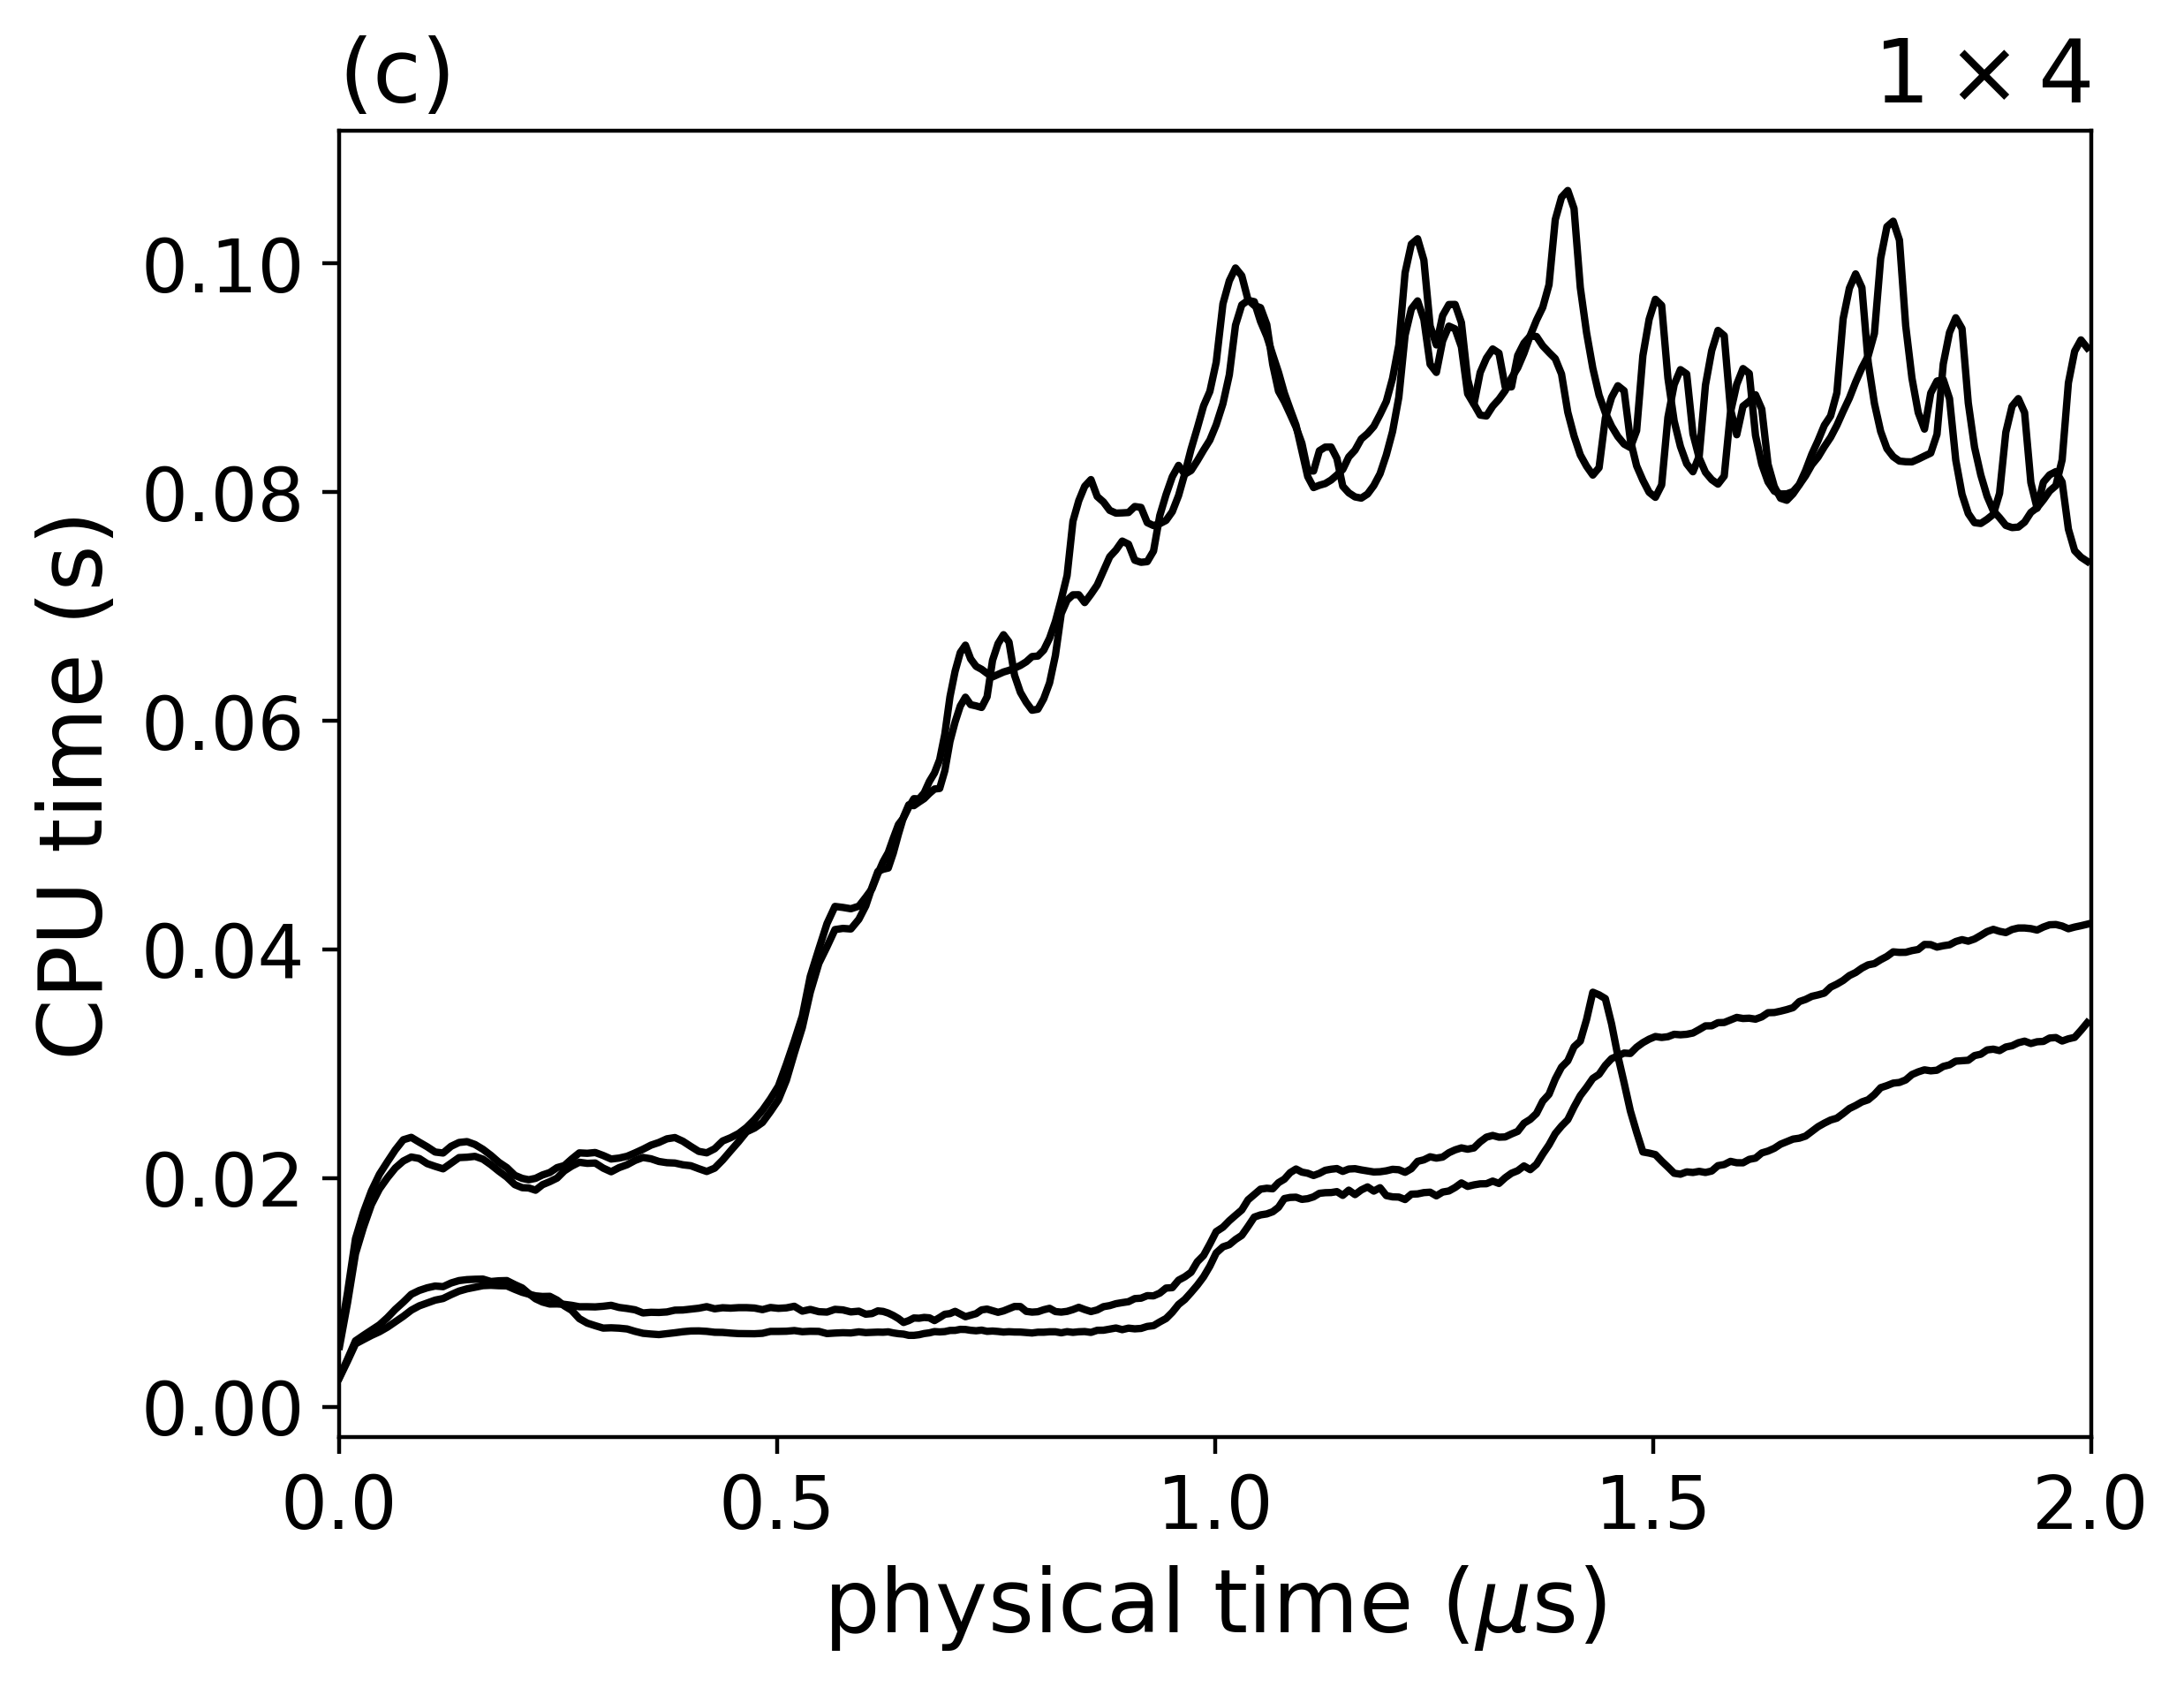
\includegraphics[width=0.45\linewidth]{time_4core_1-4.png} 
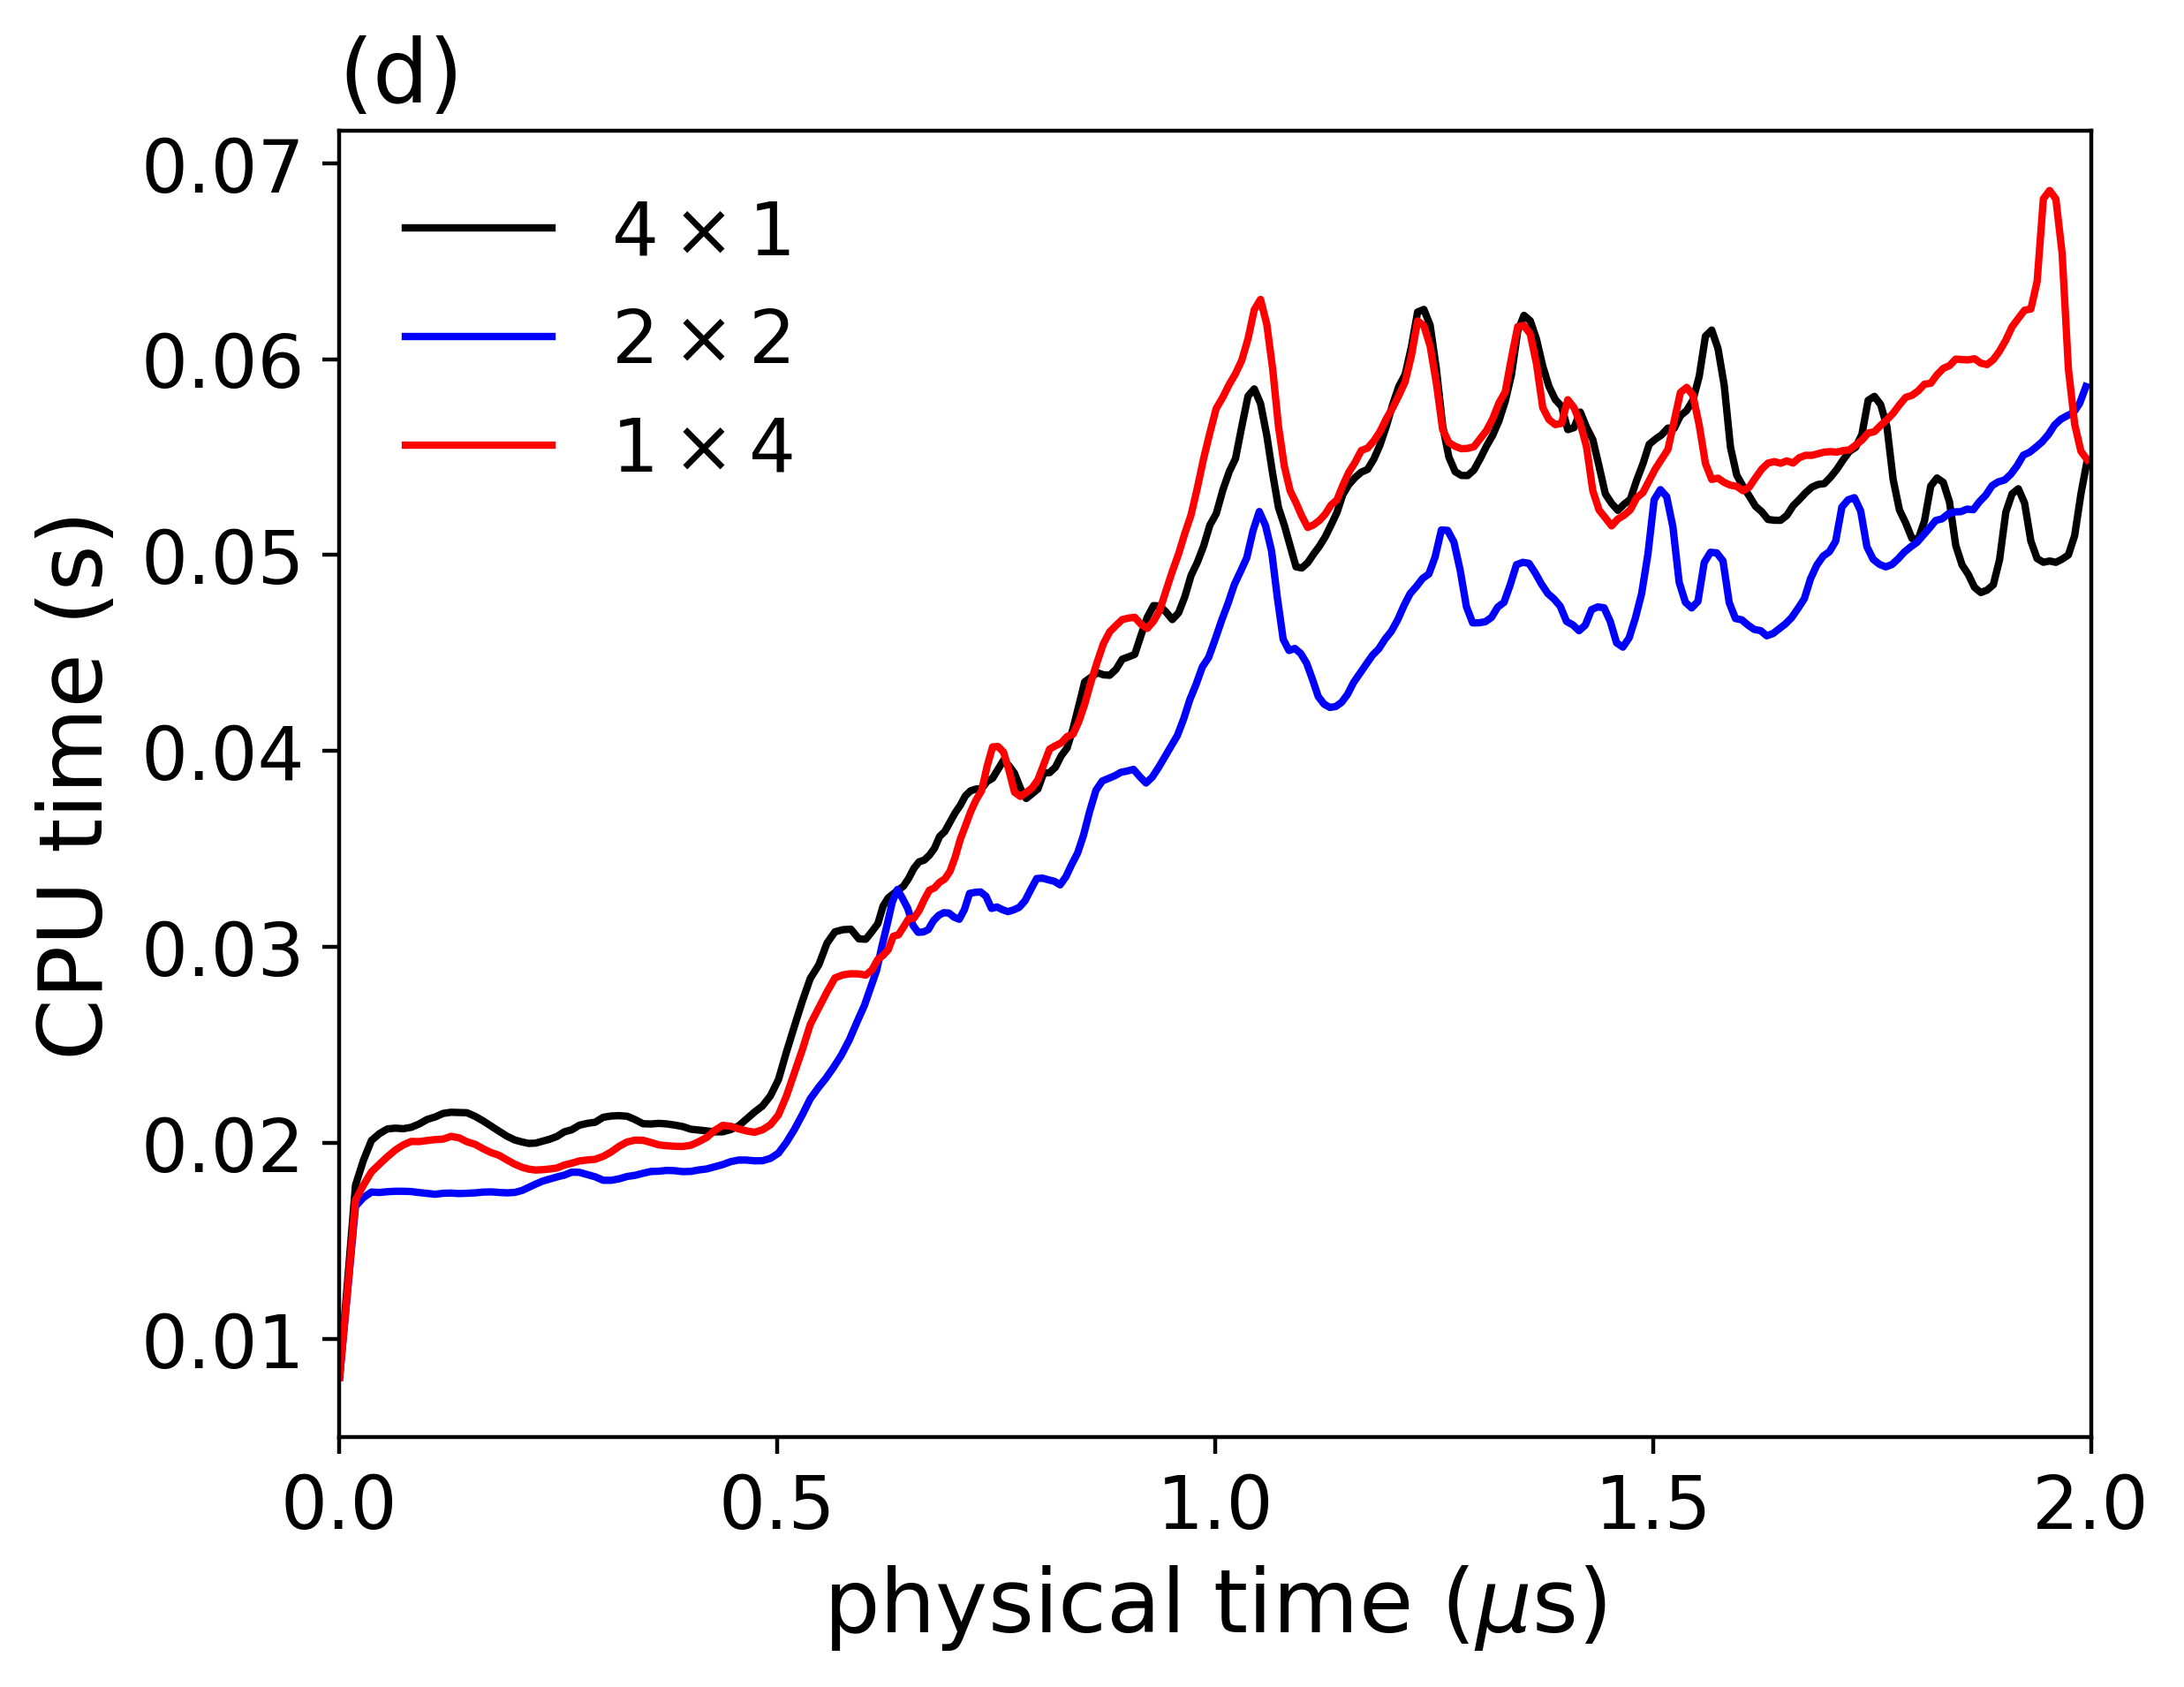
\includegraphics[width=0.45\linewidth]{time_4core_lb.png} 
\caption{The effect of domain decomposition on the ISAT performance. (a)-(c) are the CPU time of 4 MPI processes using oringal ISAT in different domain decomposition: (a) $4\times1$, (b) $2\times2$, (c) $1\times4$. (d) the CPU time using share ISAT + LB in different domain decomposition}\label{MPI_4core} 
\end{figure}

%下图展现了所有9个算例的总时间消耗,可以看出来shared ISAT 与origal ISAT 都明显的收到domain decomposition的影响,而且shared ISAT 并不总能获得相对于origal ISAT更好的性能。这是由于在shared ISAT中为了维护数据结构的完整防止data racing,我们设计的并发算法会降低一定性能,而且shared table使得table的大小增加,减慢搜索的速度。但是在shared ISAT with LB 中,性能受domain decomposition大大降低了。获得了明显的性能提升。

Fig.~\ref{MPI_4core_all} illustrates the total time consumption across all nine examples. It is evident that both shared ISAT and original ISAT are noticeably influenced by domain decomposition, and shared ISAT does not consistently outperform the original ISAT. This discrepancy arises from the fact that in shared ISAT, our concurrency algorithm, designed to maintain data structure integrity and prevent data racing, introduces some performance overhead. Additionally, the shared table increases in size, which can slow down search speeds.

However, in the case of shared ISAT with LB, domain decomposition leads to a significant performance boost. This improvement is particularly noteworthy and underscores the advantages of this specific configuration.


\begin{figure}[htbp]
    \centering
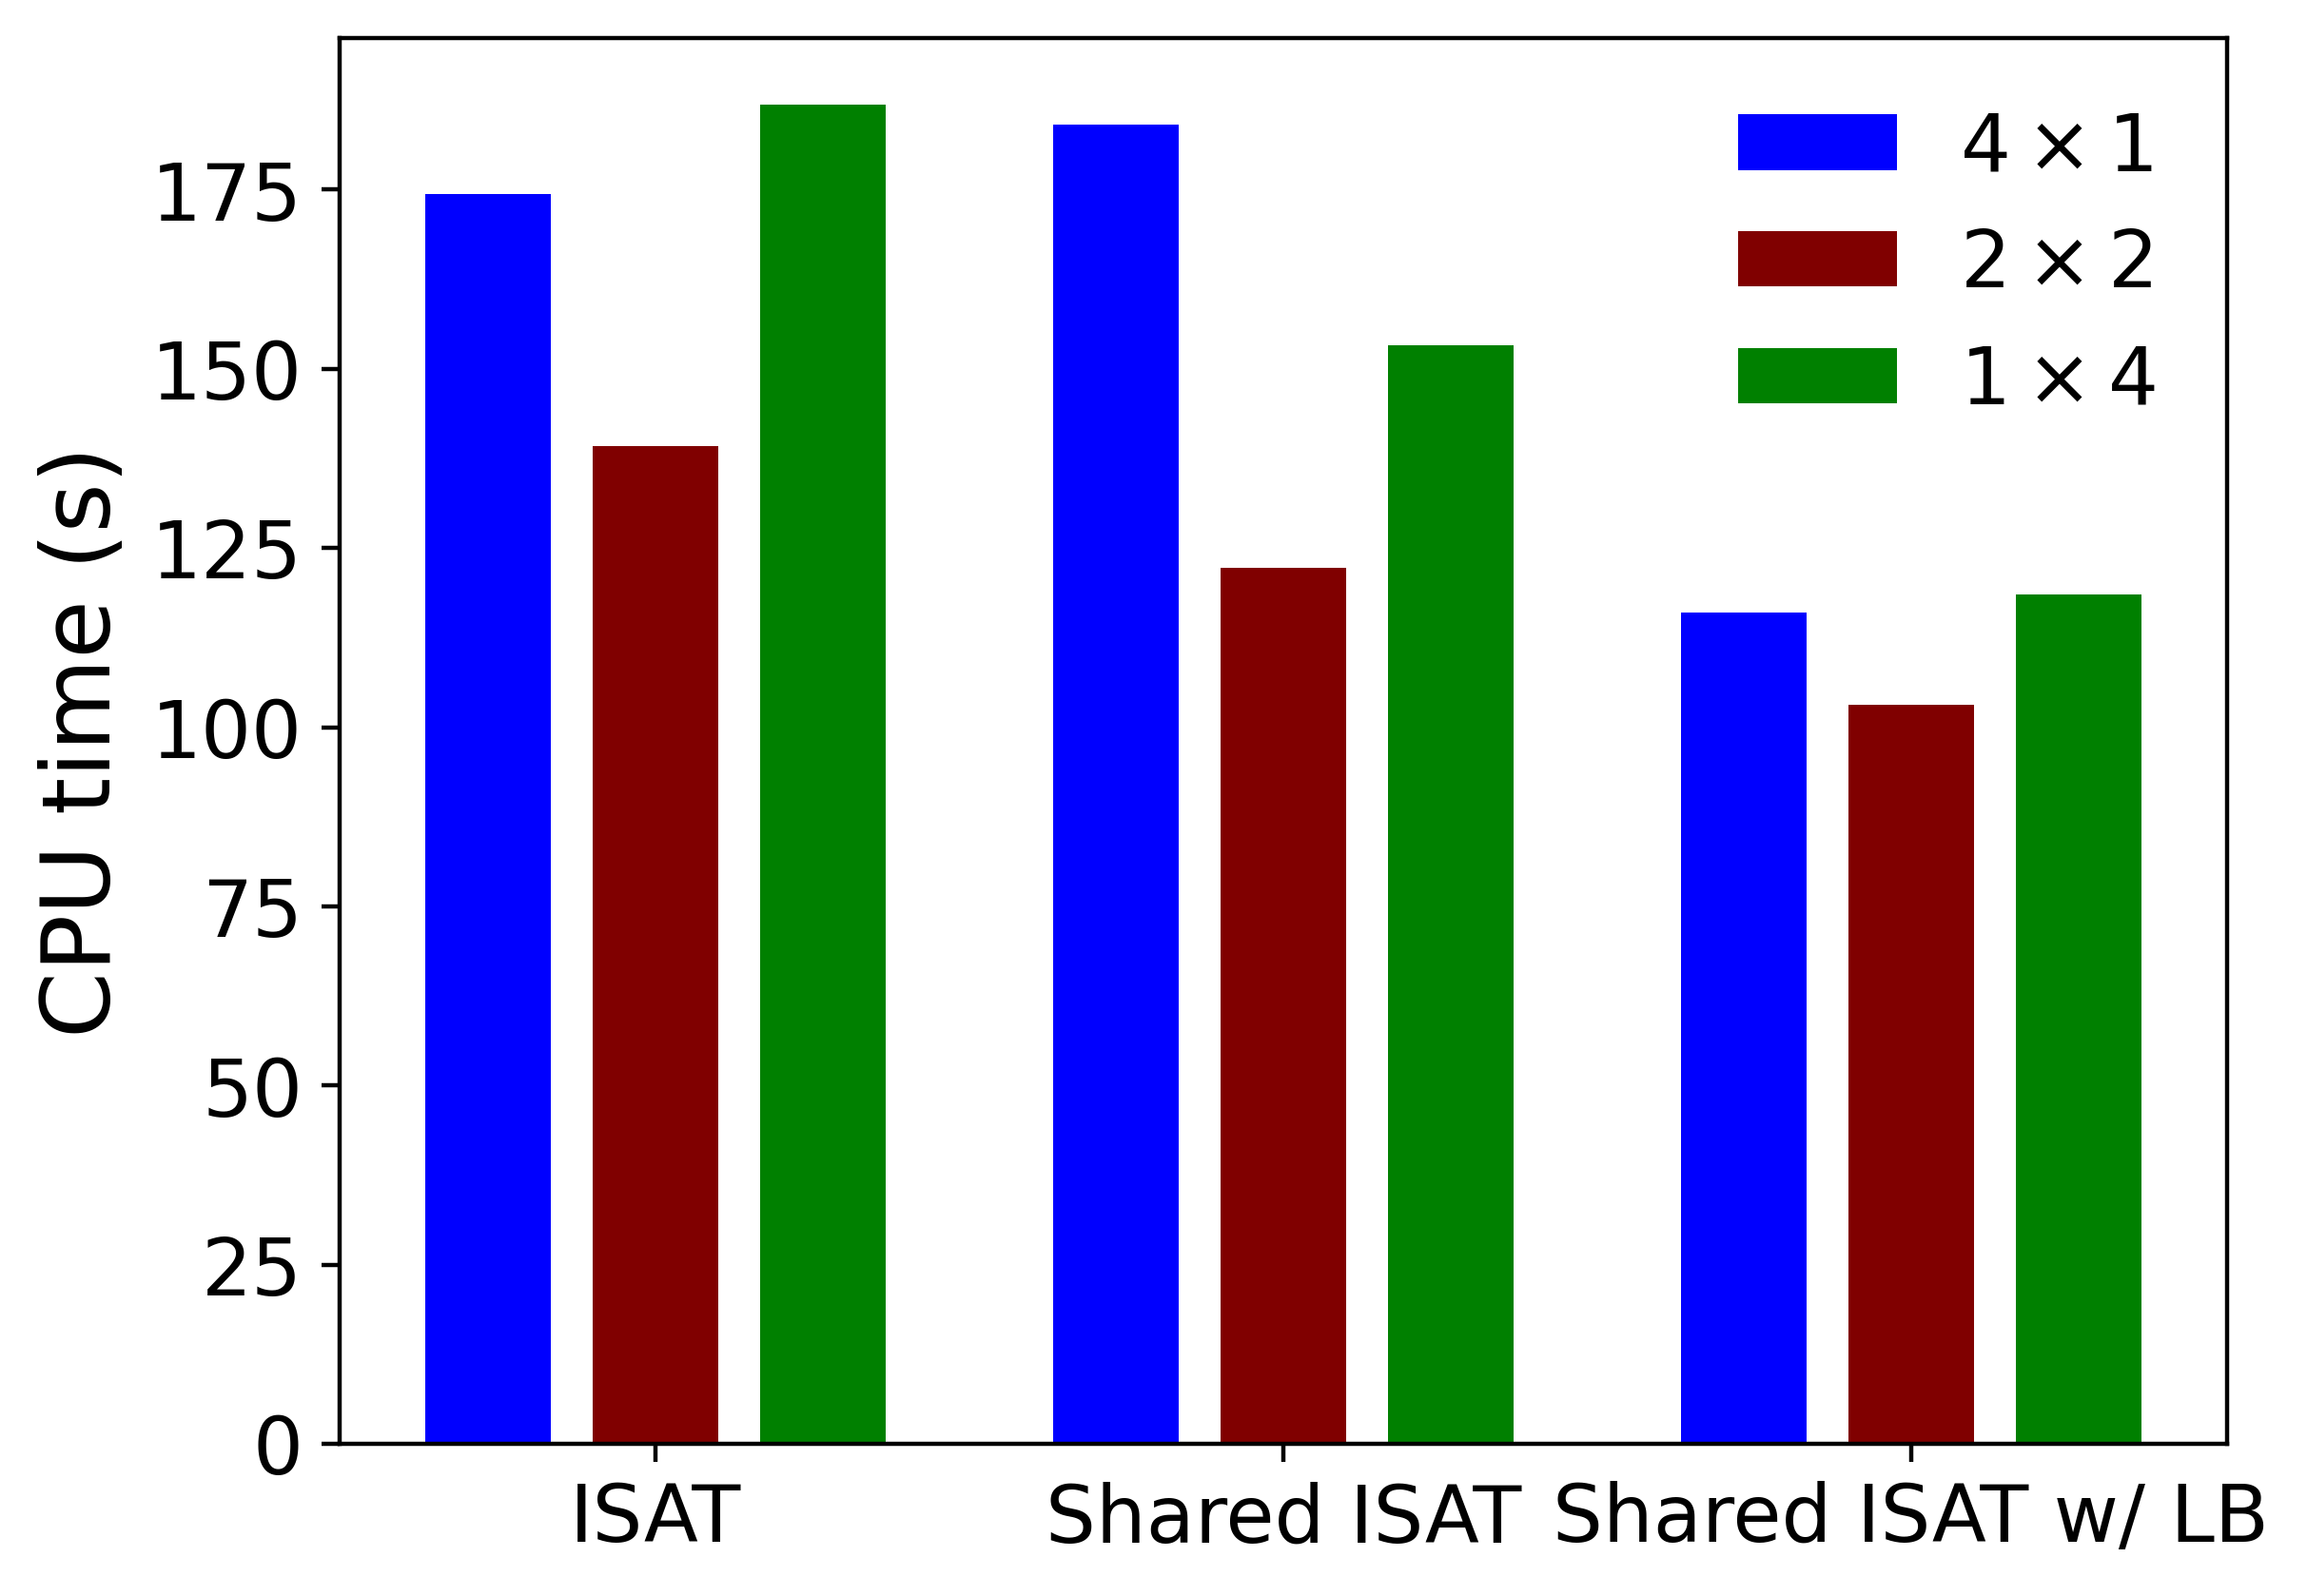
\includegraphics[width=0.45\linewidth]{time_4core_all.png} 

\caption{The effect of domain decomposition on the ISAT performance. The bar chart shows total CPU time cost of simualtions using all combination of ISAT methods and decomposition methods}\label{MPI_4core_all} 
\end{figure}

%接下来我们测试方法的scaliity, 我们选取之前使用过的3D算例,使用128x128x128的网格,计算在8,16,32,64,128核时的性能。对比在分割时尽量选取使个个维度的分割份数相同(2-2-2,4-2-2,4-4-2,4-4-4,8-4-4)。








%%%%%%%%%%%%%%%%%%%%%%%%%%%%%%%%%%%%%%%%%%%%%%%%%%%%%%%%%%%%%%%%%%%%%%%%%%%%%%%%
